%%	build-queue:
%%	
%%	¦¦¦ very first run. No .ist files yet
%%	¦¦	index, citation/bibliography or glossary changed
%%	¦	every change apart from the above mentioned. Double run for labels and toc.
%%	
%%	¦¦¦xelatex
%%	¦¦makeglossaries
%%	¦¦makeindex
%%	¦¦bibtex
%%	¦xelatex
%%	¦xelatex
%%	

\RequirePackage[l2tabu,orthodox]{nag}
\documentclass[10pt,a4paper,titlepage,twoside,english,final]{zhawreprt}

	\setdefaultlanguage{english}
\RequirePackage{lscape}
\usepackage{pgfgantt}
\usepackage{xcolor}
	\definecolor{lgray}{RGB}{250,250,250}
	\definecolor{lgreen}{RGB}{63,127,95}
	\definecolor{lred}{RGB}{127,0,85}
	\definecolor{lblue}{RGB}{42,0,255}
\usepackage{listings}
	\lstdefinestyle{basestyle}{
		basicstyle=\small\ttfamily,
		breakatwhitespace = true,
		tabsize = 4,
		frame = double,
		numbers = left,
		numbersep = 10pt,
		numberstyle = {\tiny\emptyaccsupp},
%		firstnumber = auto,
		numberblanklines = true,
		captionpos = b,
		columns = fullflexible,
		extendedchars = true,
		float = ht,
		showtabs = false,
		showspaces=false,
		showstringspaces=false,
		breaklines=true,
%		prebreak=\Righttorque
		backgroundcolor=\color{lgray},
		keywordstyle=\color{lred}\bfseries,
		commentstyle=\color{lgreen}\ttfamily,
%		morekeywords={printstr, printhexln},
		stringstyle=\color{lblue},
		xleftmargin = \fboxsep,
		xrightmargin = -6pt,
		showstringspaces=true,
	}
	\newcommand{\setlistingCSharp}{
		\lstset{
		style = basestyle,
		language = [Sharp]C,
		%otherkeywords = {*,<,>,=,;,\{,\}},
		%deletekeywords = {...},
	}}
	\newcommand{\setlistingCpp}{
		\lstset{
		style = basestyle,
		language = C++,
		%otherkeywords = {*,<,>,=,;,\{,\}},
		%deletekeywords = {...},
	}}
	\newcommand{\setlistingJava}{
		\lstset{
		style = basestyle,
		language = Java,
		%otherkeywords = {*,<,>,=,;,\{,\}},
		%deletekeywords = {...},
	}}
	\newcommand{\setlistingLaTeX}{
		\lstset{
		style = basestyle,
		language = TeX,
		%otherkeywords = {*,<,>,=,;,\{,\}},
		%deletekeywords = {...},
	}}
	\newcommand{\setlistingMatlab}{
		\lstset{
		style = basestyle,
		language = Matlab,
		otherkeywords = {methods,enumeration,properties,classdef,Sealed,Abstract},
		%deletekeywords = {...},
	}}
\usepackage{xstring}
	\newcommand{\inlist}[2]{
		\IfSubStr{,#2,}{,\arabic{#1},}{\color{lgray!95!blue}}{\color{lgray}}
	}
\usepackage{lstlinebgrd}
	\makeatletter
	\renewcommand{\lst@linebgrd}{%
	\ifx\lst@linebgrdcolor\empty\else
		\rlap{%
			\lst@basicstyle
			\color{lgray}
			\lst@linebgrdcolor{%
				\kern-\dimexpr\lst@linebgrdsep\relax%
				\lst@linebgrdcmd{\lst@linebgrdwidth}{\lst@linebgrdheight}{\lst@linebgrddepth }%
			}%
		}%
	\fi}
	\makeatother
\usepackage[space=true]{accsupp}
	\newcommand\emptyaccsupp[1]{\BeginAccSupp{ActualText={}}#1\EndAccSupp{}}
\usepackage{rotating}
\usepackage{mathptmx}
\usepackage{amssymb}
\usepackage{textcomp}
\usepackage[squaren]{SIunits}
\usepackage{amsmath}
\usepackage{amsfonts}
\usepackage{amssymb}
\usepackage[toc,page]{appendix}
\usepackage{fontspec}
	\setmainfont{Arial} % sets the roman font
	\setsansfont{Arial} % sets the sans-sérif font
	\setmonofont{Arial} % sets the monospace font
\usepackage{microtype}
\usepackage{colortbl}
\usepackage{tabularx}
\usepackage{longtable}
\usepackage{pgf,tikz}
	\usetikzlibrary{shapes}
	\usetikzlibrary{shapes.geometric}
	\usetikzlibrary{shapes.arrows}
	\usetikzlibrary{positioning}
	\usetikzlibrary{fit}
	\usetikzlibrary{calc}
	\usetikzlibrary{patterns}
\usepackage{pgfplots}
	\pgfplotsset{compat=1.13}
\usepackage{array}
\usepackage{natbib}
	\bibliographystyle{agsm}
\usepackage{usecases}
\usepackage{footnote}
	\makesavenoteenv{description}
\usepackage{makeidx}
	\makeindex
\usepackage[nottoc]{tocbibind}
\makeatletter
	\if@inltxdoc\else
	  \renewenvironment{theindex}%
	    {\if@twocolumn
	       \@restonecolfalse
	     \else
	       \@restonecoltrue
	     \fi
	     \if@bibchapter
	        \if@donumindex
	          \refstepcounter{section}
	          \twocolumn[\vspace*{2\topskip}%
	                     \@makechapterhead{\indexname}]%
	          \addcontentsline{toc}{section}{\protect\numberline{\thesection}\indexname}
	          \sectionmark{\indexname}
	        \else
	          \if@dotocind
	            \twocolumn[\vspace*{2\topskip}%
	                       \@makeschapterhead{\indexname}]%
	            \prw@mkboth{\indexname}
	            \addcontentsline{toc}{section}{\protect\numberline{\thesection}\indexname}
	          \else
	            \twocolumn[\vspace*{2\topskip}%
	                       \@makeschapterhead{\indexname}]%
	            \prw@mkboth{\indexname}
	          \fi
	        \fi
	     \else
	        \if@donumindex
	          \twocolumn[\vspace*{-1.5\topskip}%
	                     \@nameuse{\@tocextra}{\indexname}]%
	          \csname \@tocextra mark\endcsname{\indexname}
	        \else
	          \if@dotocind
	            \twocolumn[\vspace*{-1.5\topskip}%
	                       \toc@headstar{\@tocextra}{\indexname}]%
	            \prw@mkboth{\indexname}
	            \addcontentsline{toc}{\@tocextra}{\indexname}
	          \else
	            \twocolumn[\vspace*{-1.5\topskip}%
	                       \toc@headstar{\@tocextra}{\indexname}]%
	            \prw@mkboth{\indexname}
	          \fi
	        \fi
	     \fi
	   \thispagestyle{plain}\parindent\z@
	   \parskip\z@ \@plus .3\p@\relax
	   \let\item\@idxitem}
	   {\if@restonecol\onecolumn\else\clearpage\fi}
	\fi
\makeatother
\usepackage{etoolbox}
\makeatletter
%	\renewcommand\listoftables{%
%	    \section{Tabellenverzeichnis}%
%	    \@mkboth{\MakeUppercase\listtablename}%
%	        {\MakeUppercase\listtablename}%
%	    \@starttoc{lot}%
%	}
%	\renewcommand\listoffigures{%
%	    \section{Abbildungsverzeichnis}%
%	    \@mkboth{\MakeUppercase\listfigurename}%
%	        {\MakeUppercase\listfigurename}%
%	    \@starttoc{lof}%
%	}
%	\renewcommand\lstlistoflistings{%
%	    \section{Listingverzeichnis}%
%	    \@mkboth{\MakeUppercase\listfigurename}%
%	        {\MakeUppercase\listfigurename}%
%	    \@starttoc{lol}%
%	}
	\renewenvironment{thebibliography}[1]
	     {\section{\bibname}% <-- this line was changed from \chapter* to \section*
	      \@mkboth{\MakeUppercase\bibname}{\MakeUppercase\bibname}%
	      \list{\@biblabel{\@arabic\c@enumiv}}%
	           {\settowidth\labelwidth{\@biblabel{#1}}%
	            \leftmargin\labelwidth
	            \advance\leftmargin\labelsep
	            \@openbib@code
	            \usecounter{enumiv}%
	            \let\p@enumiv\@empty
	            \renewcommand\theenumiv{\@arabic\c@enumiv}}%
	      \sloppy
	      \clubpenalty4000
	      \@clubpenalty \clubpenalty
	      \widowpenalty4000%
	      \sfcode`\.\@m}
	     {\def\@noitemerr
	       {\@latex@warning{Empty `thebibliography' environment}}%
	      \endlist}
\makeatother
	
	\renewcommand\appendixname{Appendix}
\makeatletter
	\renewenvironment{theindex}{
		\renameindex
		\let\ps@plainorig\ps@plain
		\let\ps@plain\ps@scrheadings
		\if@twocolumn
			\@restonecolfalse
		\else
			\@restonecoltrue
		\fi
		\columnseprule \z@
		\columnsep 35\p@
		\twocolumn[\section{\indexname}]%
		\@mkboth{\MakeUppercase\indexname}{\MakeUppercase\indexname}%
		\thispagestyle{plain}\parindent\z@
		\parskip\z@ \@plus .3\p@\relax
	\let\item\@idxitem}
	{\if@restonecol\onecolumn\else\clearpage\fi}
\makeatother

\usepackage{varioref}
\usepackage[colorlinks=true, linkcolor=black, citecolor=black, plainpages=false, unicode, pdfencoding=auto ,backref=page]{hyperref}
\usepackage{cleveref}
\usepackage[automake,acronym,numberedsection]{glossaries-extra}
	\renewcommand*{\glspostdescription}{}
	\newglossary[slg]{symbols}{sym}{sbl}{List of Symbols}
	\makeglossaries
	\loadglsentries{glossaryentries.tex}
	\pdfstringdefDisableCommands{\let\textenglish\@firstofone\let\textgerman\@firstofone}
	\makeatletter
	\renewcommand*{\@@glossarysec}{section}
	\makeatother
\if false
\newcommand{\FullGlossaryEntry}[7]{%Abkz., Typ, Name, Name(plural), Beschr., Beschr.(plural), Erkl.
\newglossaryentry{#1}{type=\acronymtype,
	name={#3},
	plural={#4},
	description={\textit{#5}},
	%first={\textit{#5}(later referred to as #3)\glsadd{_#1}},
	%firstplural={\textit{#6}(later referred to as #4)\glsadd{_#1}},
	first={#5 (#3)\glsadd{_#1}},
	firstplural={#6 (#4)\glsadd{_#1}},
	see=[See]{_#1}
}
\longnewglossaryentry{_#1}{type=#2,
	name={#5},
	plural={#6}
	}{\hspace{0pt}\\#7}
}


% Acronyms
%\newacronym{jlu}{JLU}{Justus-Liebig-Universität}
%\newacronym{hrz}{HRZ}{Hochschulrechenzentrum}
%\newacronym[plural=LEDs, longplural={light-emitting diodes}]{led}{LED}{light-emitting diode}
%\newacronym[plural=EEPROMs, longplural={electrically erasable programmable read-only memories}]{eeprom}{EEPROM}{electrically erasable programmable read-only memory}

%  Glossary Entries
\newglossaryentry{port}{
	name=port,
	description={A point for traffic to flow, represented by an unsigned integer of up to 2 bytes. The name was chosen as an analogy to ports for ships.},
	plural=ports
}
\newglossaryentry{shell}{
	name=shell,
	description={A \gls{CLI} program, that reads user input line-by-line and executes those commands.},
	plural=shells
}
\newglossaryentry{loopback}{
	name=loopback,
	description={A channel with only one endpoint: Sender and receiver are on the same machine.},
	plural=loopbacks
}
\newglossaryentry{pipe}{
	name=pipe,
	description={A pipe is a \gls{Unix} feature for \gls{IPC}.},
	plural=pipes
}
\newglossaryentry{socket}{
	name=socket,
	description={A network socket is an endpoint for communication over \glspl{port}.},
	plural=sockets
}
\newglossaryentry{uptime}{
	name=uptime,
	description={The time a computer has been running.}
}
\newglossaryentry{login}{
	name=login,
	description={The action of logging in.}
	plural=logins
}
\newglossaryentry{terminal}{
	name=terminal,
	description={An user interface to interact with \gls{CLI} programs like \glspl{shell}.},
	plural=terminals
}
\newglossaryentry{Unix}{
	name=Unix,
	description={An originally free \gls{OS} family called Unics from AT\&T that re-imagined an older \gls{OS} by the name of Multics.}
}
\newglossaryentry{Linux}{
	name=Linux,
	description={A \gls{Unix} based \gls{OS} which uses Linus Torvalds kernel and was inspired by Minix.}
}
\newglossaryentry{daemon}{
	name=daemon,
	description={A (possibly latent) background process on a \gls{Unix} machine that handles certain events when said events occur.},
	plural=daemons
}
\newglossaryentry{Request Broker}{
	name=Request Broker,
	description={A service that oversees the action requests of a program and decides whether to permit and execute them or not, based on various factors.},
	plural=Request Brockers
}

\newglossaryentry{CGo}{
	name=CGo,
	description={\gls{C} support for \gls{Go}.}
}
\newglossaryentry{x-package}{
	name=x-package,
	description={A \gls{Go} package that is not part of the standard library and that is subject to change or even entirely disappear.}
	plural=x-packages
}
\newglossaryentry{X.509}{
	name=X.509,
	description={An international standard for certificates in public key infrastructures.}
}
\newglossaryentry{DiffieHellmanKX}{
	name={Diffie-Hellman key exchange},
	description={A key exchange algorithm that prevents exposure to eavesdropping third parties.},
	plural={Diffie-Hellman key exchanges}
}

% Acronyms
\newglossaryentry{OS}{type=\acronymtype,
name={OS},
plural={OSes},
description={\textit{Operating System}},
first={Operating System(OS)},
firstplural={Operating Systems(OSes)}
}

% Acronyms with Glossary Entries
\FullGlossaryEntry{ZHAW}{main}%
{ZHAW}{}%
{Zurich University of Applied Sciences}{}%
{Name of my university of trust.}

\FullGlossaryEntry{Go}{main}%
{Go}{}%
{the Go/Golang programming language}{}%
{Google's programming language.}

\FullGlossaryEntry{C}{main}%
{C}{}%
{the C programming language}{}%
{Low-level programming language originally invented by Dennis Ritchie.}

\FullGlossaryEntry{C++}{main}%
{C++}{}%
{the C++ programming language}{}%
{Descendant of \gls{C} which implemented \gls{OOP}.}

\FullGlossaryEntry{OOP}{main}%
{OOP}{}%
{Object Oriented Programming}{}%
{A programming paradigm which uses objects to model real life entities.}

\FullGlossaryEntry{fd}{main}%
{fd}{fds}%
{file descriptor}{file descriptors}%
{A file descriptor is an integer that represents the handle to a file.}

\FullGlossaryEntry{CLI}{main}%
{CLI}{}%
{Command Line Interface}{}%
{A text based interface centered around commands to perform specific tasks.}

\FullGlossaryEntry{tty}{main}%
{tty}{ttys}%
{teletype}{teletypes}%
{Originally a device that could send and receive text messages. Nowadays \gls{tty} refers to \glspl{terminal}, which emulate that behaviour \citep{tty}.}

\FullGlossaryEntry{pty}{main}%
{pty}{ptys}%
{pseudoterminal}{pseudoterminals}%
{A mechanism of \gls{Unix} to allow programs to communicate as if the other was inside a \gls{tty} \citep{pty}.}

\FullGlossaryEntry{ptm}{main}%
{ptm}{ptms}%
{pseudoterminal master}{pseudoterminal masters}%
{The master of a \gls{pty}.}

\FullGlossaryEntry{pts}{main}%
{pts}{pts's}%
{pseudoterminal slave}{pseudoterminal slaves}%
{The slave of a \gls{pty} \citep{pts}.}

\FullGlossaryEntry{SIGINT}{main}%
{\texttt{SIGINT}}{\texttt{SIGINT}s}%
{interrupt signal}{interrupt signals}%
{A signal supported by \gls{Unix} based \glspl{OS} which signals to a process to interrupt it's work.}

\FullGlossaryEntry{SIGWINCH}{main}%
{\texttt{SIGWINCH}}{\texttt{SIGWINCH}s}%
{window change signal}{window change signals}%
{A signal supported by \gls{Unix} based \glspl{OS} which signals to a process that the terminal window it is running in has changed size.}

\FullGlossaryEntry{SSH}{main}%
{SSH}{}%
{Secure Shell}{}%
{An client-server-application that allows remote login and interaction with a \gls{shell}. See \ref{sec:OpenSSH}.}

\FullGlossaryEntry{PAM}{main}%
{PAM}{PAMs}%
{Pluggable Authentication Module}{Pluggable Authentication Modules}%
{Modules for user authentication.}

\FullGlossaryEntry{API}{main}%
{API}{APIs}%
{Application Programming Interface}{Application Programming Interfaces}%
{Accessible interface for developers to use external code.}

\FullGlossaryEntry{PID}{main}%
{PID}{PIDs}%
{Process ID}{Process IDs}%
{The unique identifier of a process represented as an integer.}

\FullGlossaryEntry{UID}{main}%
{UID}{UIDs}%
{User ID}{User IDs}%
{The unique identifier of a user represented as an integer.}

\FullGlossaryEntry{GID}{main}%
{GID}{GIDs}%
{Group ID}{Group IDs}%
{The unique identifier of a group represented as an integer.}

\FullGlossaryEntry{SID}{main}%
{SID}{SIDs}%
{Session ID}{Session IDs}%
{The unique identifier of a session represented as an integer.}

\FullGlossaryEntry{IPC}{main}%
{IPC}{}%
{Inter-Process-Communication}{}%
{Communication between processes.}

\FullGlossaryEntry{GUI}{main}%
{GUI}{GUIs}%
{Graphical User Interface}{Graphical User Interfaces}%
{Graphical interface for the user to visually interact with a program.}

\FullGlossaryEntry{SSL}{main}%
{SSL}{}%
{Secure Sockets Layer}{}%
{Cryptographic protocol to secure the communication between two peers via symmetric cryptography. Deprecated.}

\FullGlossaryEntry{TLS}{main}%
{TLS}{}%
{Transport Layer Security}{}%
{Newer and recommended version of \gls{SSL}.}

\FullGlossaryEntry{TELNETS}{main}%
{TELNETS}{}%
{Telnet Secure}{}%
{Telnet with \gls{SSL} encryption.}

\FullGlossaryEntry{WSL}{main}%
{WSL}{}%
{Windows Subsystem for Linux}{}%
{A subsystem provided by Windows that is able to run headless \gls{Linux} distributions.}

\FullGlossaryEntry{NIS}{main}%
{NIS}{}%
{Network Information Service}{}%
{A service for distributing configurations like user information among a network.}

\FullGlossaryEntry{LDAP}{main}%
{LDAP}{}%
{Lightweight Directory Access Protocol}{}%
{A protocol for querying and managing information of distributed directory information services.}


% Symbols
%\newglossaryentry{ohm}{type=symbols, name={\ensuremath{\Omega}}, sort=Ohm, symbol={\ensuremath{\Omega}}, description={unit of electrical resistance}}
%\newglossaryentry{angstrom}{type=symbols, name={\AA}, sort=angström, symbol={\AA}, description={non-SI unit of length}}
\fi

\logofilename{images/logos/SoE/de/de-soe-cmyk.png}
\projecttype{PA}
\major{HS16 Studiengang Informatik}
\title{Spaghetti Bolognese mit Parmesan}
\shorttitle{Spaghetti}
\author{Raphael Emberger}
\authors{Raphael Emberger, Kal-El,\\Musashi Miyamoto}
\mainreferee{}
\referee{}
\industrypartner{}
\extreferee{}
\setdate{\today}

\begin{document}

\maketitle

\chapter*{Abstract}\label{sec:Abstract}
\notes{\item Zusammenfassung}


\chapter*{Preface}\label{sec:Preface}
\notes{\item Stellt den persönlichen Bezug zur Arbeit dar und spricht Dank aus.}
The \gls{SSH} protocol \citep{rfc253,rfc6668,rfc8268,rfc8308,rfc8332} is a system that allows a user to log in on a remote machine and perform tasks on that remote machine via a \gls{CLI}. \gls{SSH} is widely known and used in everyday tasks. However: It is now over twelve years old in its current form. One of the problems with \gls{SSH} is its complexity, both in the initial phase when key material is exchanged, but also later, for example because the server must always decide whether to return a character that has been sent to it or not (echo).

The goal of this work is a radically simplified protocol, which in its functions is similar to \gls{SSH} (N.B. the similarity concerns the functions, not necessarily the protocol details). I develop the protocol, as well as a client and a server - all in \gls{Go}. I demonstrate that the software can replace \gls{SSH} by showing that it can handle several common use cases, among them:

\begin{itemize}
\item Interactive session
\item \texttt{Rsync} with my solution as transport protocol
\end{itemize}

This bachelor thesis was proposed by Dr. Stephan Neuhaus \citep{BA19_neut_03} and aroused my interest as it is a challenge in the domain of information security and will produce a palpable result.

On this note I would like to thank \gls{ZHAW} for granting me the opportunity to do my Bachelors thesis here and Dr. Stephan Neuhaus for helping me along the way of this Bachelors thesis.

\makedeclarationoforiginality

\tableofcontents

\chapter{Introduction}\label{chp:Introduction}
\section{Initial Position}\label{sec:InitialPosition}
\notes{
\item Nennt bestehende Arbeiten/Literatur zum Thema -> Literaturrecherche
\item Stand der Technik: Bisherige Lösungen des Problems und deren Grenzen
\item (Nennt kurz den Industriepartner und/oder weitere Kooperationspartner und dessen/deren Interesse am Thema Fragestellung)
}
There was no thesis done on this subject that could have been used as reference. There are however several software projects that deal with a similar problem.

\subsection{OpenSSH}\label{ssec:OpenSSH}
The most noteworthy work to mention is of course \gls{SSH} itself. \cite{openssh} is the name of the open source project which provides millions of administrators and developers with the ability to securely connect to a remote host. It replaces the up until then widely used protocols like \cite{telnet}(see \ref{ssec:Telnet}) and \cite{rlogin}/\cite{rsh}(see \ref{ssec:BerkeleyRCommands}).\\
\gls{SSH} uses \gls{TLS} to secure the communication channel between two peers and has earned itself a spot on the low end of the \gls{port} table: It occupies \gls{port} 22.\\
\gls{SSH}s features can be used very flexibly: After it builds up a secure connection between a client and a server, it can be used to remotely login and use a \gls{terminal} on that machine.
It can also forward traffic on local ports to the remote host through the secure channel. This is also used by third party programs such as \cite{rsync}.\\
When it comes to the log in procedure itself, \gls{SSH} allows for standard user log in using the \gls{API} of the \glspl{PAM}. Another feature is whitelisting of clients via their public keys, which barres intrusion via hijacked user-password-credentials.\\
After a secure connection could be established, there are multiple possibilities to use the opened channel. One is to forward the \gls{GUI} of a remote program to the client. Another one is to use this channel to tunnel more connections through it: For example can the traffic of an application which uses a specific \gls{port} be forwarded to the remote host. This can obscure and secure this traffic between the host and the server.

\subsection{Telnet}\label{ssec:Telnet}
Telnet\citep{rfc15,rfc854} is an old(1969) and deprecated communication protocol which doesn't feature any security. However, in other implementations, \gls{TELNETS} was proposed, which features encryption over the communication channel.\\
Telnet still has 23 as its very own \gls{port} assigned to it.
\subsubsection{Go-Telnet}
Go-Telnet\citep{gotelnet} is a \gls{TELNETS} supporting client-server-application which has been implemented in \gls{Go}.

\subsection{Berkeley r-commands}\label{ssec:BerkeleyRCommands}
The Berkley r-commands are a set of commands to do certain tasks on remote hosts. Those tasks are similar to their counterparts without a leading "\texttt{r}".
\begin{itemize}
\item \cite{rlogin}\\
This command connects to the host and performs a \cite{login} command, which includes authentication and if successful, spawning a user \gls{shell}.
\item \cite{rsh}\\
\texttt{rsh} spawns a \gls{shell} without the log in process.
\item \cite{rexec}\\
With this command, the user can log in to a remote machine and execute one command.
\item \cite{rcp}\\
Using this command gives the user the ability to copy from and to a remote host.
\item \cite{rwho}\\
This command tells the user what users are currently logged in on the remote machine.
\item \cite{rstat}\\
\texttt{rstat} displays file system information from remote hosts.
\item \cite{ruptime}\\
With this command, the user can see the uptime, number of logged in users and current work load of the remote machine.
\end{itemize}


\section{Task}\label{sec:Task}
\notes{
\item Formuliert das Ziel der Arbeit
\item Verweist auf die offizielle Aufgabenstellung des/der Dozierenden im Anhang
\item (Pflichtenheft, Spezifikation)
\item (Spezifiziert die Anforderungen an das Resultat der Arbeit)
\item (Übersicht über die Arbeit: stellt die folgenden Teile der Arbeit kurz vor)
\item (Angaben zum Zielpublikum: nennt das für die Arbeit vorausgesetzte Wissen)
\item (Terminologie: Definiert die in der Arbeit verwendeten Begriffe)
}
The official formulation of the tasks can be found in the appendix \ref{ssec:OfficialStatementOfTasks}.\\
The objective of this thesis is as follows:
\begin{itemize}
\item Design and implementation of a client-server protocol that can manage interactive sessions.
\item Design and implementation of a privilege-separation architecture on the server side that allows safe dropping of privileges once a client establishes a connection.
\end{itemize}

For a passing grade (4.0), the work must contain at least the following:
\begin{itemize}
\item In the thesis, an introduction to the problem and why the envisaged solution will solve it.
\item In the thesis, a survey of related work in the area.
\item In the thesis, a detailed design of the solution.
\item In the thesis, an evaluation of the performance of the implemented solution.
\item In the software, a privilege-separation architecture.
\end{itemize}

Incorporating the following components will improve the grade:
\begin{itemize}
\item In the related work section of the thesis, a comparison of all the related work with the envisaged solution, outlining why the envisaged solution is better.
\item In the thesis, a detailed analysis of the security of the solution, including possible attacks and defenses.
\item Use of \gls{TLS} as the transport layer.
\item A proof-of-concept client that can handle interactive sessions.
\item A proof-of-concept client that works as a transport for \texttt{rsync}.
\end{itemize}

\vspace{1.5cm}
This thesis has been worded with technically literate readers in mind. However: For core concepts and special terms, a glossary can be found at \ref{sec:Glossary}. Used acronyms are listed in \ref{sec:AcronymGlossary}.

\chapter{Design}\label{chp:Design}
\section{Implementation Language}\label{sec:ImplementationLanguage}
In the beginning of the project, Dr Neuhaus suggested the use of \gls{Go} as a modern low-level language over interpreted languages for considerations of security. He emphasized that the use of other low-level languages(like \gls{C} or \gls{C++}) was permissible. In the end the project was implemented in \gls{Go} as suggested.\\
However, this lead to a few problems in the implementation process(See \ref{sec:Problems}).

\section{Authentication via PAM}\label{sec:AuthViaPAM}
For authentication of users on Linux systems, \gls{PAM} exists. I provides a clean separation between a program and the sensitive part of authentication. \gls{PAM} operates using transactions, which represent a link to a \gls{PAM} context. Using this transaction, an application can do various actions regarding account management, authentication or session management. To initialize such a context and transaction, an application has to call the \cite{pam_start} function.
\setlistingC
\begin{lstlisting}[caption={Initializing a \gls{PAM} context},label=lst:InitPAMContext]
#include <security/pam_appl.h>

struct pam_message {
    int msg_style;
    const char *msg;
};

struct pam_response {
    char *resp;
    int resp_retcode;
};

struct pam_conv {
    int (*conv)(int num_msg, const struct pam_message **msg,
                struct pam_response **resp, void *appdata_ptr);
    void *appdata_ptr;
};
int pam_start(const char *service_name, const char *user, const struct pam_conv *pam_conversation, pam_handle_t **pamh);
\end{lstlisting}

Similarly, the created context has to be terminated with \cite{pam_end}
\setlistingC
\begin{lstlisting}[caption={Terminating a \gls{PAM} context},label=lst:TermPAMContext]
#include <security/pam_appl.h>

int pam_end(pam_handle_t *pamh, int pam_status);
\end{lstlisting}

After creating a context, the application can prepare the transaction with \cite{pam_set_item} and \cite{pam_get_item}. Using those function, fields like \texttt{PAM\_RUSER} and \texttt{PAM\_RHOST}, which together(\texttt{PAM\_RUSER@PAM\_RHOST}) represent the requesting user(remote or local). If in any of the prior or later steps any errors occur, the corresponding error message can be received with \cite{pam_strerror}.
\setlistingC
\begin{lstlisting}[caption={\gls{PAM} functions},label=lst:PAMFunctions]
#include <security/pam_appl.h>

int pam_get_item(const pam_handle_t *pamh, int item_type, const void **item);
int pam_set_item(pam_handle_t *pamh, int item_type, const void *item);
const char *pam_strerror(pam_handle_t *pamh, int errnum);
\end{lstlisting}

Now that the transaction has been appropriately prepared, the application can request to authenticate a user via \cite{pam_authenticate}:
\setlistingC
\begin{lstlisting}[caption={\gls{PAM} authentication},label=lst:PAMAuthentication]
#include <security/pam_appl.h>

int pam_authenticate(pam_handle_t *pamh, int flags);
\end{lstlisting}

Now \gls{PAM} uses the \texttt{pam\_conv} struct given in \cite{pam_start} that points to a function to interactively ask the application to authenticate the user. The application can then ask the user for the user name if not provided already and the password. After successful authentication, the function returns \texttt{PAM\_SUCCESS} and the application should call \cite{pam_setcred} to establish and maintain the credentials of the logged in user.
\setlistingC
\begin{lstlisting}[caption={\gls{PAM} credential setting},label=lst:PAMCredSet]
#include <security/pam_appl.h>

int pam_setcred(pam_handle_t *pamh, int flags);
\end{lstlisting}

Now the application can do other \gls{PAM} related actions like session management(see \ref{ssec:LoginAccountingWithPAM}). To finish, the application terminates the context properly and all associated memory gets invalidated.

\section{Authentication via Keys}\label{sec:AuthViaKeys}
A user can also authenticate himself without a password but instead using public key cryptography. For this, a user has to create a key pair consisting of a private and a public key. Before the actual authentication, a hashed version of the public key has to be stored on the server.\\
When starting an authentication, the user sends his public key to the server, which compares its hash with the stored keys that are deemed permissible for authentication. If it matches, the server encrypts a random secret(with high entropy) with the public key to the user. The user decrypts the message with his private key and sends it back to the server. If the returned secret matches the original secret, the user proved that he is the legitimate owner of the public key.\\
This authentication is sufficiently secure from third parties which do not have access to the private key of the user, as it can prove the authenticity of a user.

\section{Post-Login Actions}\label{sec:PostLoginActions}
When a user logs into a \gls{Unix} machine, a session and a timestamp gets created.\\
For this, the two files \texttt{/var/run/utmp} and \texttt{/var/log/wtmp} provide the appropriate storage. The \texttt{utmpx} \gls{API} offers appropriate functions. The \texttt{utmpx} struct represents a single entry in those files:
\setlistingC
\begin{lstlisting}[caption={Definition of the utmpx structure {\citep[p.819]{KerriskTLPI}}},label=lst:UtmpxDefinition]
#define _GNU_SOURCE
/* Without _GNU_SOURCE the two field names below are prepended by "__" */
struct exit_status {
	short e_termination; /* Process termination status (signal) */
	short e_exit; 		 /* Process exit status */
};
#define __UT_LINESIZE 32
#define __UT_NAMESIZE 32
#define __UT_HOSTSIZE 256
struct utmpx {
	short ut_type; 				 /* Type of record */
	pid_t ut_pid; 				 /* PID of login process */
	char ut_line[__UT_LINESIZE]; /* Terminal device name */
	char ut_id[4]; 				 /* Suffix from terminal name, or	ID field from inittab(5) */
	char ut_user[__UT_NAMESIZE]; /* Username */
	char ut_host[__UT_HOSTSIZE]; /* Hostname for remote login, or kernel version for run-level messages */
	struct exit_status ut_exit;  /* Exit status of process marked as DEAD_PROCESS (not filled in by init(8) on Linux) */
	long ut_session; 			 /* Session ID */
	struct timeval ut_tv; 		 /* Time when entry was made */
	int32_t ut_addr_v6[4]; 		 /* IP address of remote host (IPv4 address uses just ut_addr_v6[0], with other elements set to 0) */
	char __unused[20]; 			 /* Reserved for future use */
};
\end{lstlisting}

On login, a record has to be written to the \texttt{utmp} file to indicate that the user logged in. If there is already a record for the active \gls{terminal}, then the entry has to be updated, otherwise a new entry has to be appended. A call to \cite{pututxline} should suffice in performing these steps properly. The application has to set the \texttt{ut\_type} field of the \texttt{ùtmpx} struct to \texttt{USER\_PROCESS} to mark a user login.\\
Similarly to the \texttt{utmp} update after login, the application has to report to the \texttt{utmpx} \gls{API} that the session ended. This procedure consists of almost the same actions as the one after login, with exception of \texttt{ut\_user} being zeroed out and \texttt{ut\_type} being set to \texttt{DEAD\_PROCESS}\citep[p.828]{KerriskTLPI}.\\
A program can also query the \texttt{utmp} file with the according getters.
\setlistingC
\begin{lstlisting}[caption={\texttt{utmpx} \gls{API} functions},label=lst:UtmpxApiFunctions]
#include <utmp.h>

struct utmp *getutent(void);
struct utmp *getutid(const struct utmp *ut);
struct utmp *getutline(const struct utmp *ut);

struct utmp *pututline(const struct utmp *ut);
\end{lstlisting}

\subsection{Login Accounting with PAM}\label{ssec:LoginAccountingWithPAM}
\gls{PAM} supports binding login accounting to its own session functions \cite{pam_open_session} and \cite{pam_close_session}:
\setlistingC
\begin{lstlisting}[caption={\gls{PAM} session management},label=lst:PAMSessionManagement]
#include <security/pam_appl.h>

int pam_open_session(pam_handle_t *pamh, int flags);
int pam_close_session(pam_handle_t *pamh, int flags);
\end{lstlisting}

\section{Terminal Mode}\label{sec:TerminalMode}
The client expects to send all its input directly to the \gls{shell} without prior interpretation. To achieve this, the client-side \gls{terminal} has to be set from the default \texttt{cooked}- into the \texttt{raw}-mode\citep[p.1309]{KerriskTLPI}. This sends each key stroke to the server-side \gls{shell} as is. After the termination of the session, the original \texttt{cooked}-mode has to be restored to ensure operation as per usual.

\section{Pseudoterminal}\label{sec:Pseudoterminal}
\glspl{pty} are an \gls{IPC} mechanism that help solving the problem of how two remote programs can communicate as if they were directly connected via a \gls{terminal}(see figure \ref{fig:HowToOperateTtyOrientedProgramOverNetwork}).\\
A \gls{shell} expects to be connected to a full fledged \gls{tty}(or a \gls{tty} emulator). To check whether it is inside such an environment, it uses \cite{isatty} on the \gls{fd} it is connected to. Therefore the \gls{fd} it is connected to should behave like a real \gls{terminal}. This is where \glspl{pty} come into play.
\begin{figure}[ht]
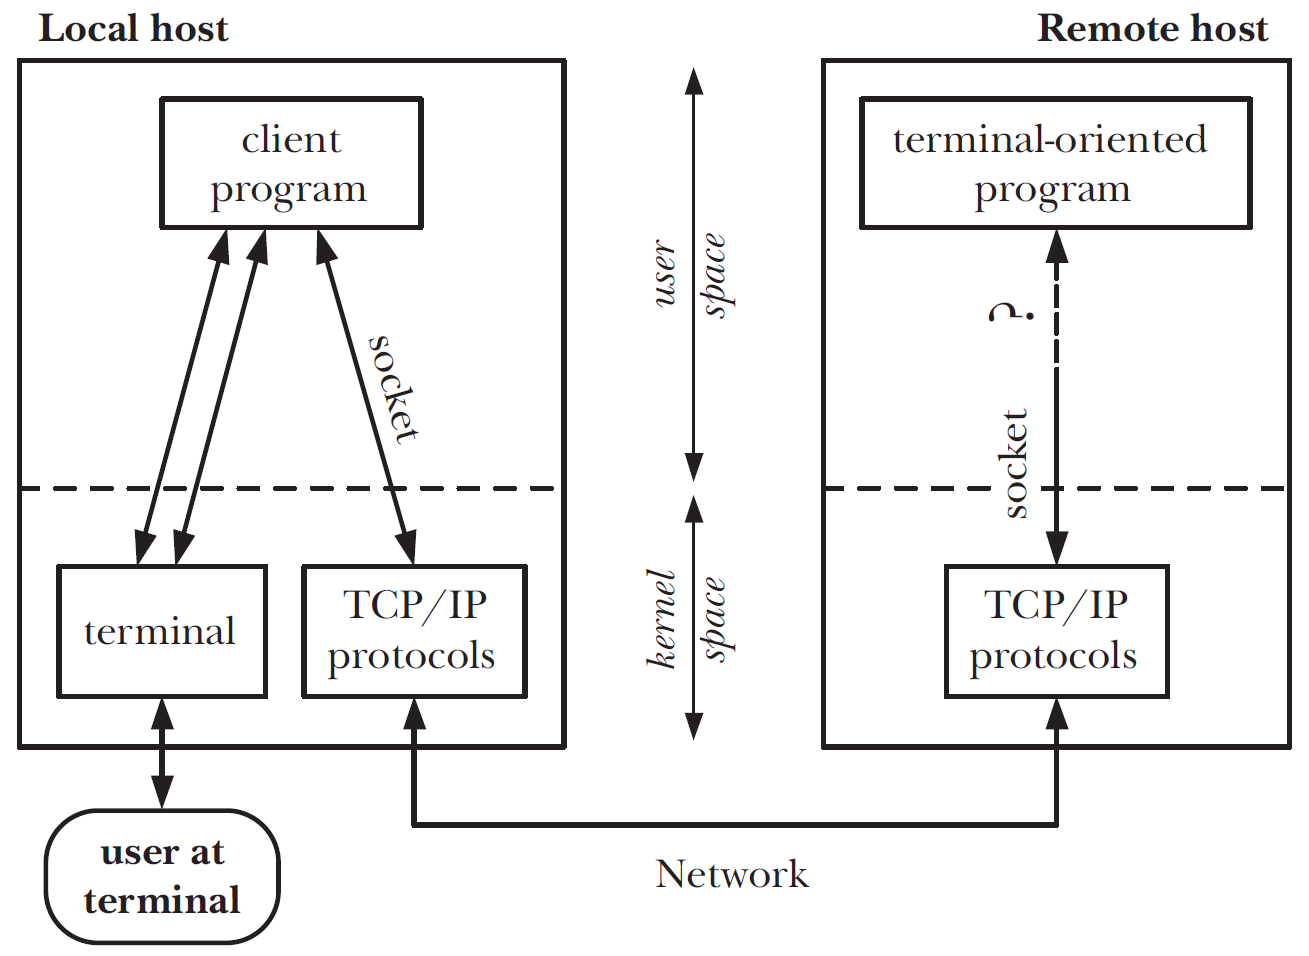
\includegraphics[width=\textwidth]{PseudoterminalProblem}
\caption{How to operate a \gls{tty}-oriented program over a network?\citep[p.1376]{KerriskTLPI}}
\label{fig:HowToOperateTtyOrientedProgramOverNetwork}
\end{figure}
\begin{figure}[ht]
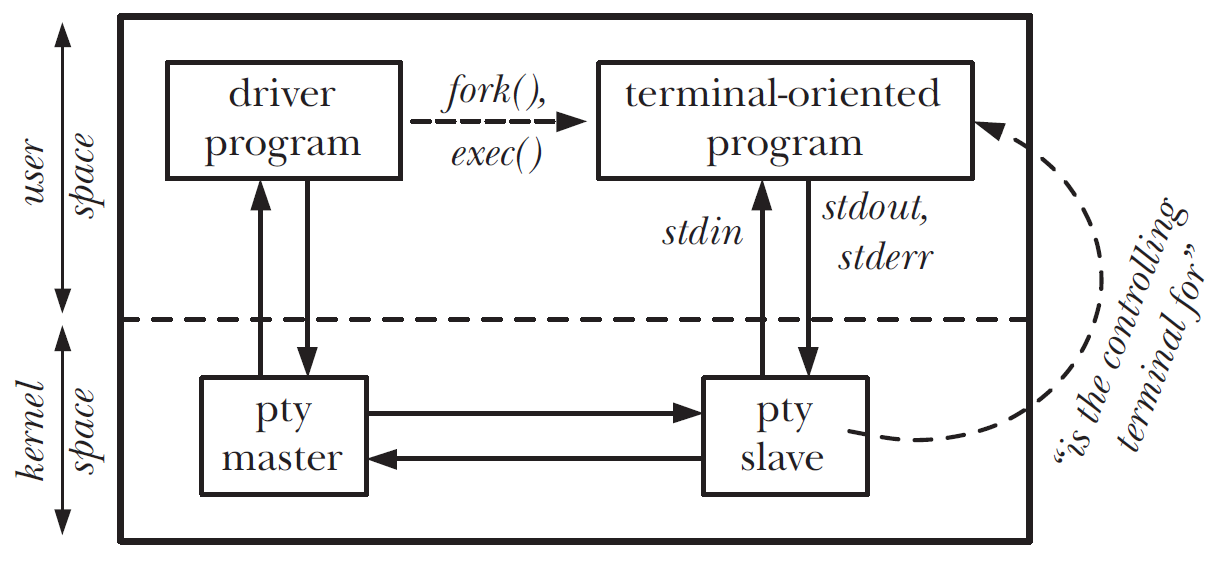
\includegraphics[width=\textwidth]{Pseudoterminal}
\caption{Two programs communicating via a \gls{pty}\citep[p.1377]{KerriskTLPI}}
\label{fig:TwoProgramsCommunicatingViaAPty}
\end{figure}
To do this, two files are created: The \gls{ptm} and the corresponding \gls{pts}(see figure \ref{fig:TwoProgramsCommunicatingViaAPty}). \gls{Linux} provides a \gls{pty} generator at \texttt{/dev/ptmx}, which creates a \gls{ptm} and a \gls{pts}. This works by simply opening the \texttt{/dev/ptmx} file using \cite{posix_openpt}. After this, a program has to grant the \gls{pts} file ownership and permissions with \cite{grantpt}, unlock it with \cite{unlockpt} and retrieve its file name with \cite{ptsname}:
\setlistingC
\begin{lstlisting}[caption={\gls{pty} related \gls{Linux} \gls{API} functions},label=lst:PtyFunctions]
#define _XOPEN_SOURCE 500
#include <stdlib.h>

int posix_openpt(int flags);
int grantpt(int fd);
int unlockpt(int fd);
char *ptsname(int fd);
\end{lstlisting}

With the \gls{pty} properly set up, a child bound to the \gls{pts} side will assume it is connected to a \gls{terminal} and also behave as such. This mechanism is key to running a \gls{shell} and forwarding all traffic between a remote client and the \gls{shell}. In case of \gls{SSH} and the objective of this thesis, the layout looks like in figure \ref{fig:HowSSHUsesPty}.
\begin{figure}[ht]
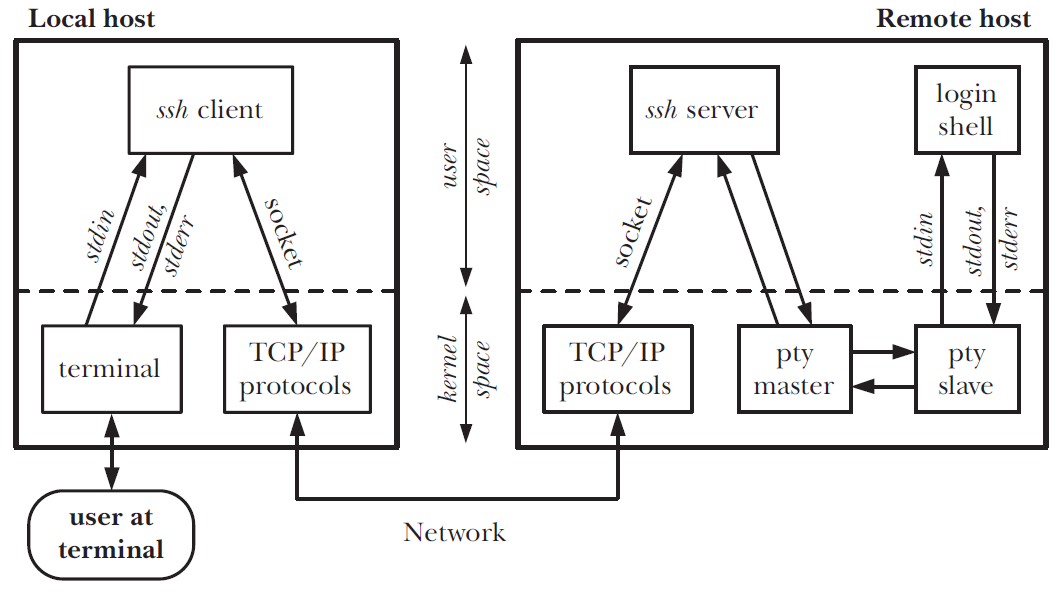
\includegraphics[width=\textwidth]{PseudoterminalSSH}
\caption{How \texttt{ssh} uses a \gls{pty}\citep[p.1378]{KerriskTLPI}}
\label{fig:HowSSHUsesPty}
\end{figure}

\newpage
\section{Flow of Action}\label{sec:FlowOfAction}
To create a client-server protocol for remote log in and interactive sessions, a clear cut architecture is mandatory. The flow of a typical use case should look like this:

\begin{enumerate}
\item Server listens for incoming connection.
\item Client dials server.
\item Server spawns the users login \gls{shell} and forwards all traffic between \gls{shell} and Client.
\item Client uses \gls{shell} on remote machine.
\item Client terminates session.
\item Host terminates.
\end{enumerate}

However, there are multiple security concerns to be satiated:

\begin{enumerate}
\item The Client must authenticate itself for a user of the remote system with the appropriate credentials.
\item The Server has to drop privilege after a successful login to prevent privilege escalation.
\item The Server has to spawn the login \gls{shell} of the logged in user with the appropriate rights.
\end{enumerate}

Furthermore, the current design does not allow for multiple sessions to be run parallel. Therefore it was decided to spawn a new process to handle everything beginning after the connection has been established.\\
This lead to  the following general flow of actions:

\begin{enumerate}
\item Server listens for incoming connection.
\item Client dials server.
\item Server spawns a Host upon established connection.
\item Host sets up connection.
\item Host asks Client to authenticate himself.
\item Client authenticates himself.
\item Host drops privilege to logged in user.
\item Host spawns the users login \gls{shell} with the same credentials and forwards all traffic between \gls{shell} and Client.
\item Client uses \gls{shell} on remote machine.
\item Client terminates session.
\item Host terminates.
\end{enumerate}

\newpage
\subsection{Old Design}\label{ssec:OldDesign}
An earlier draft of the flow of actions was designed as a sequence diagram and can be seen in figure \ref{fig:SeqDiaOriginal}.
\begin{figure}[ht]
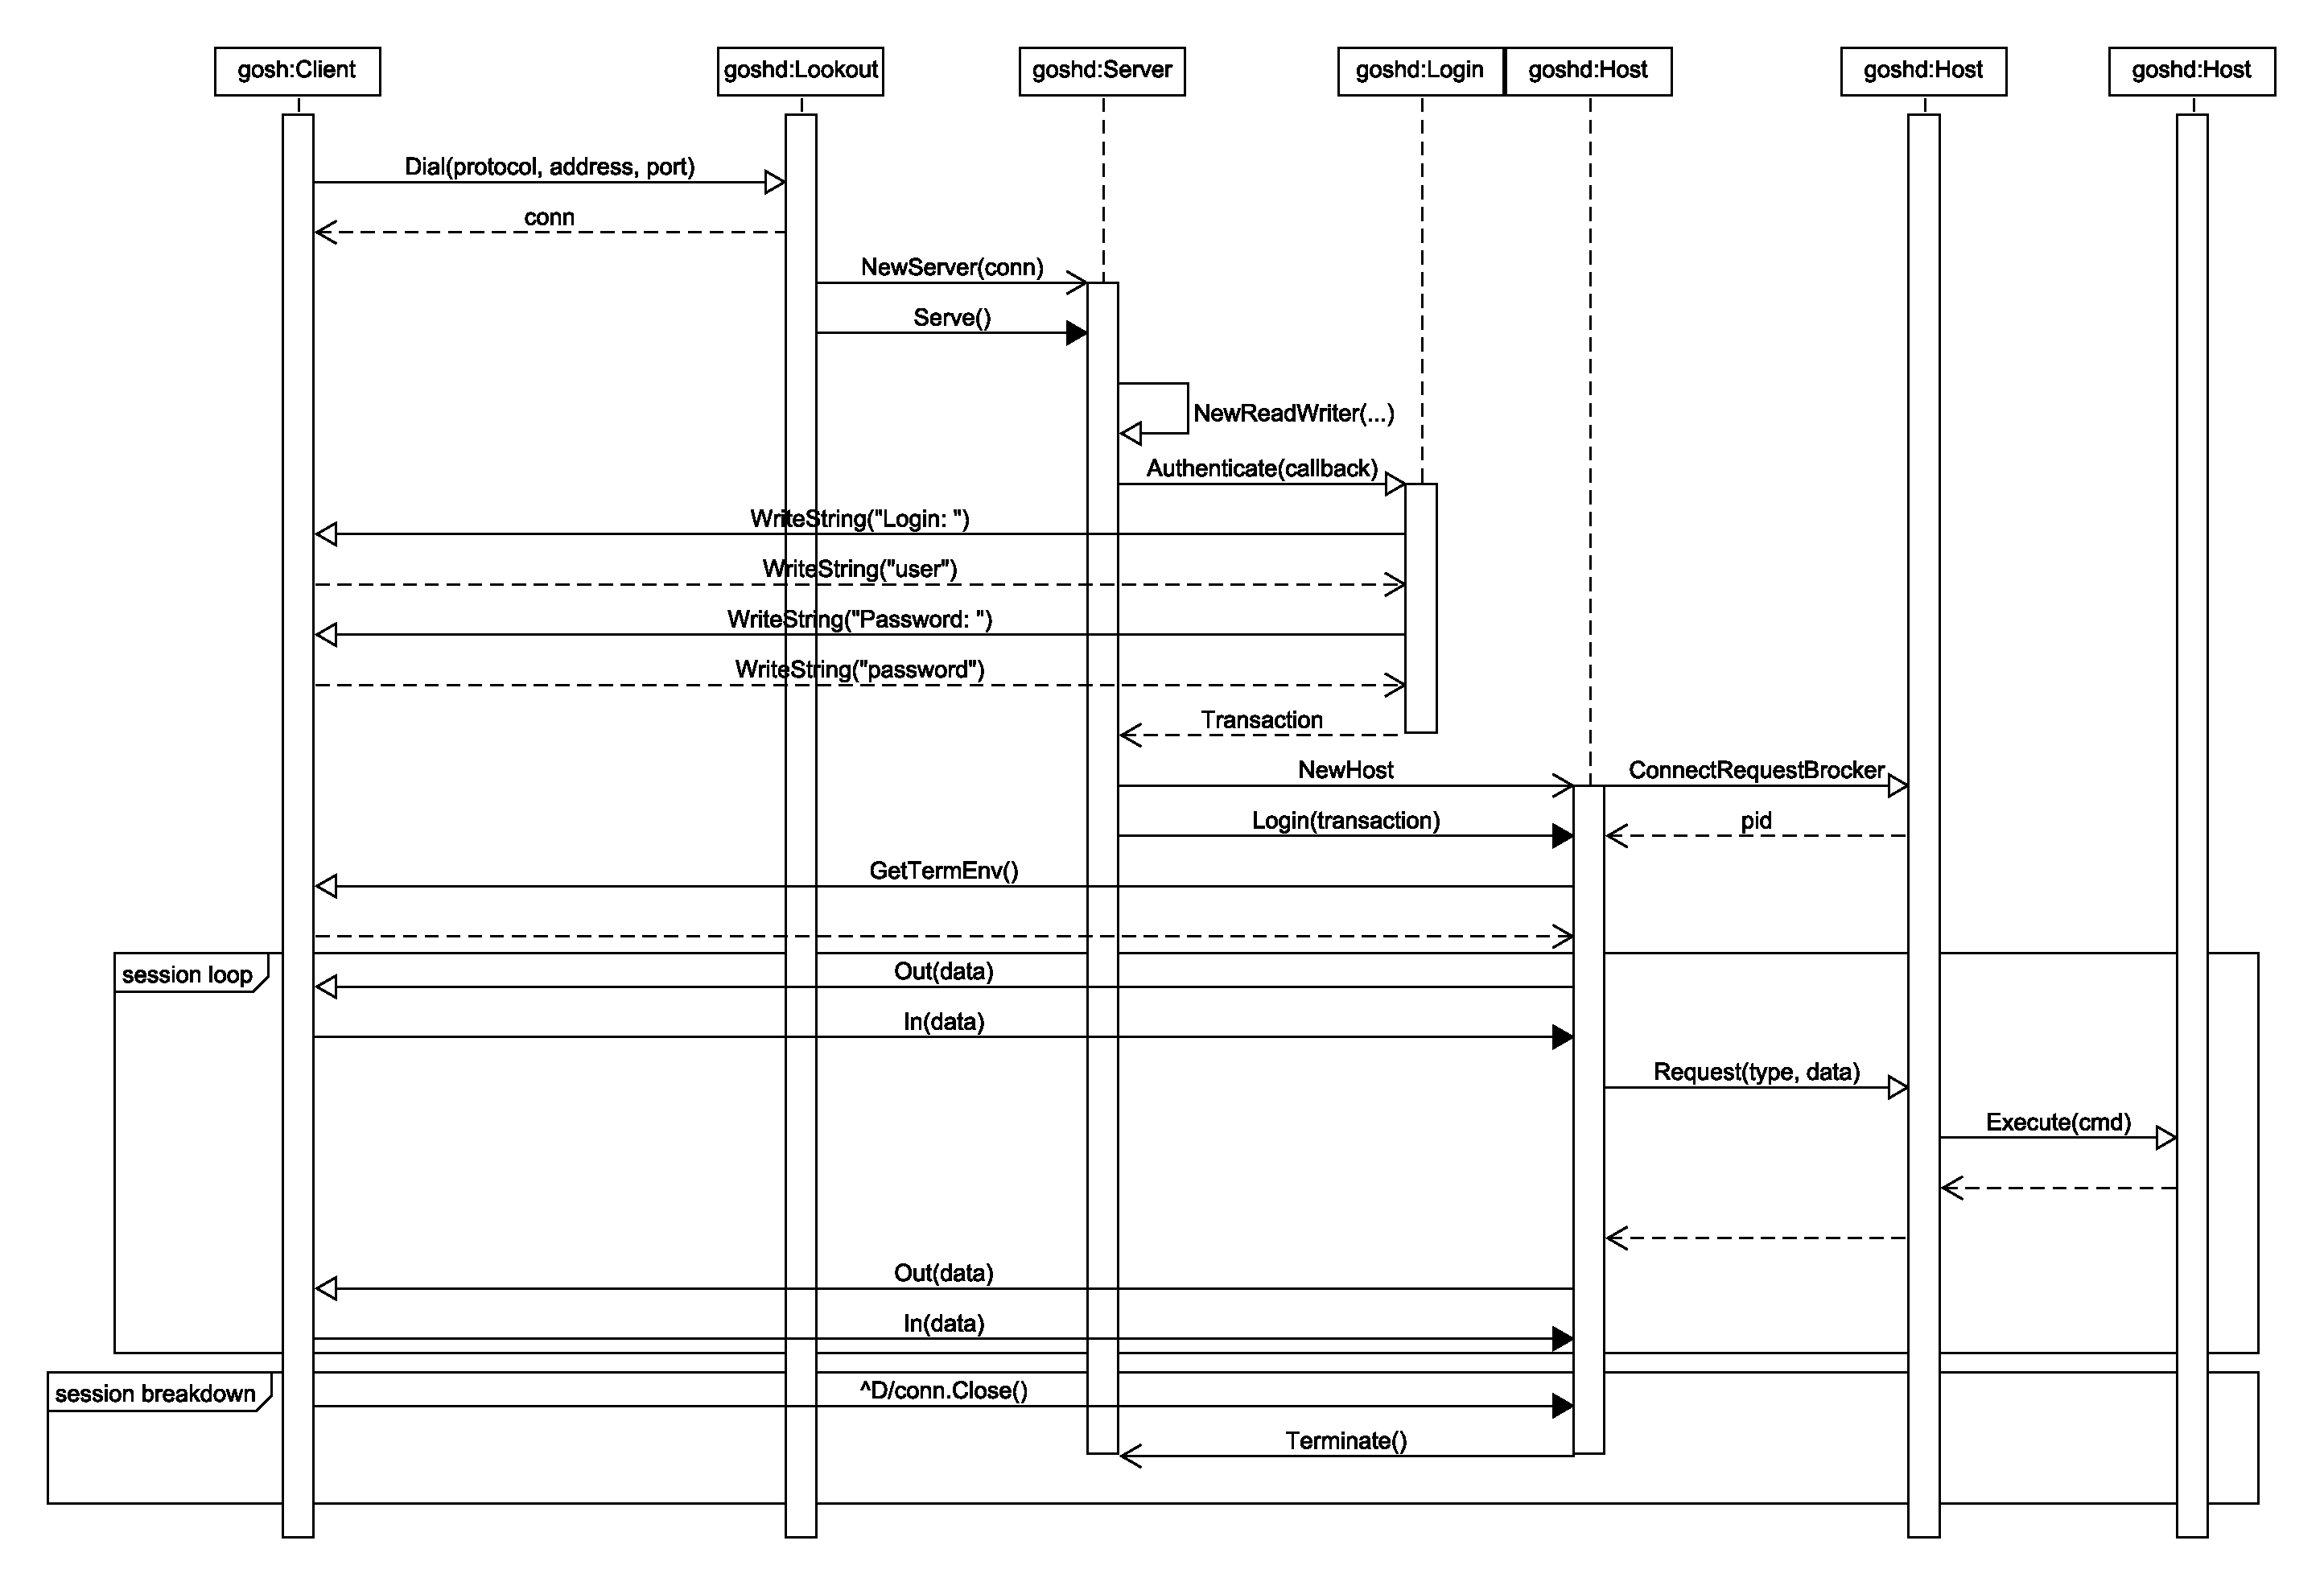
\includegraphics[width=\textwidth]{SequenceDiagram}
\caption{Sequence diagram draft.}
\label{fig:SeqDiaOriginal}
\end{figure}

This design used a \gls{Request Broker}, which would put another master-slave-relationship between a \gls{shell} and the \gls{Request Broker}. This would have been an over-complication of the use of a \gls{shell}, which, if set correctly, already runs only with the rights of the corresponding user and its groups.

\subsection{New Design}\label{ssec:NewDesign}
The new and current design of the architecture can be seen in figure \ref{fig:SeqDiaCurrent}.
\begin{figure}[ht]
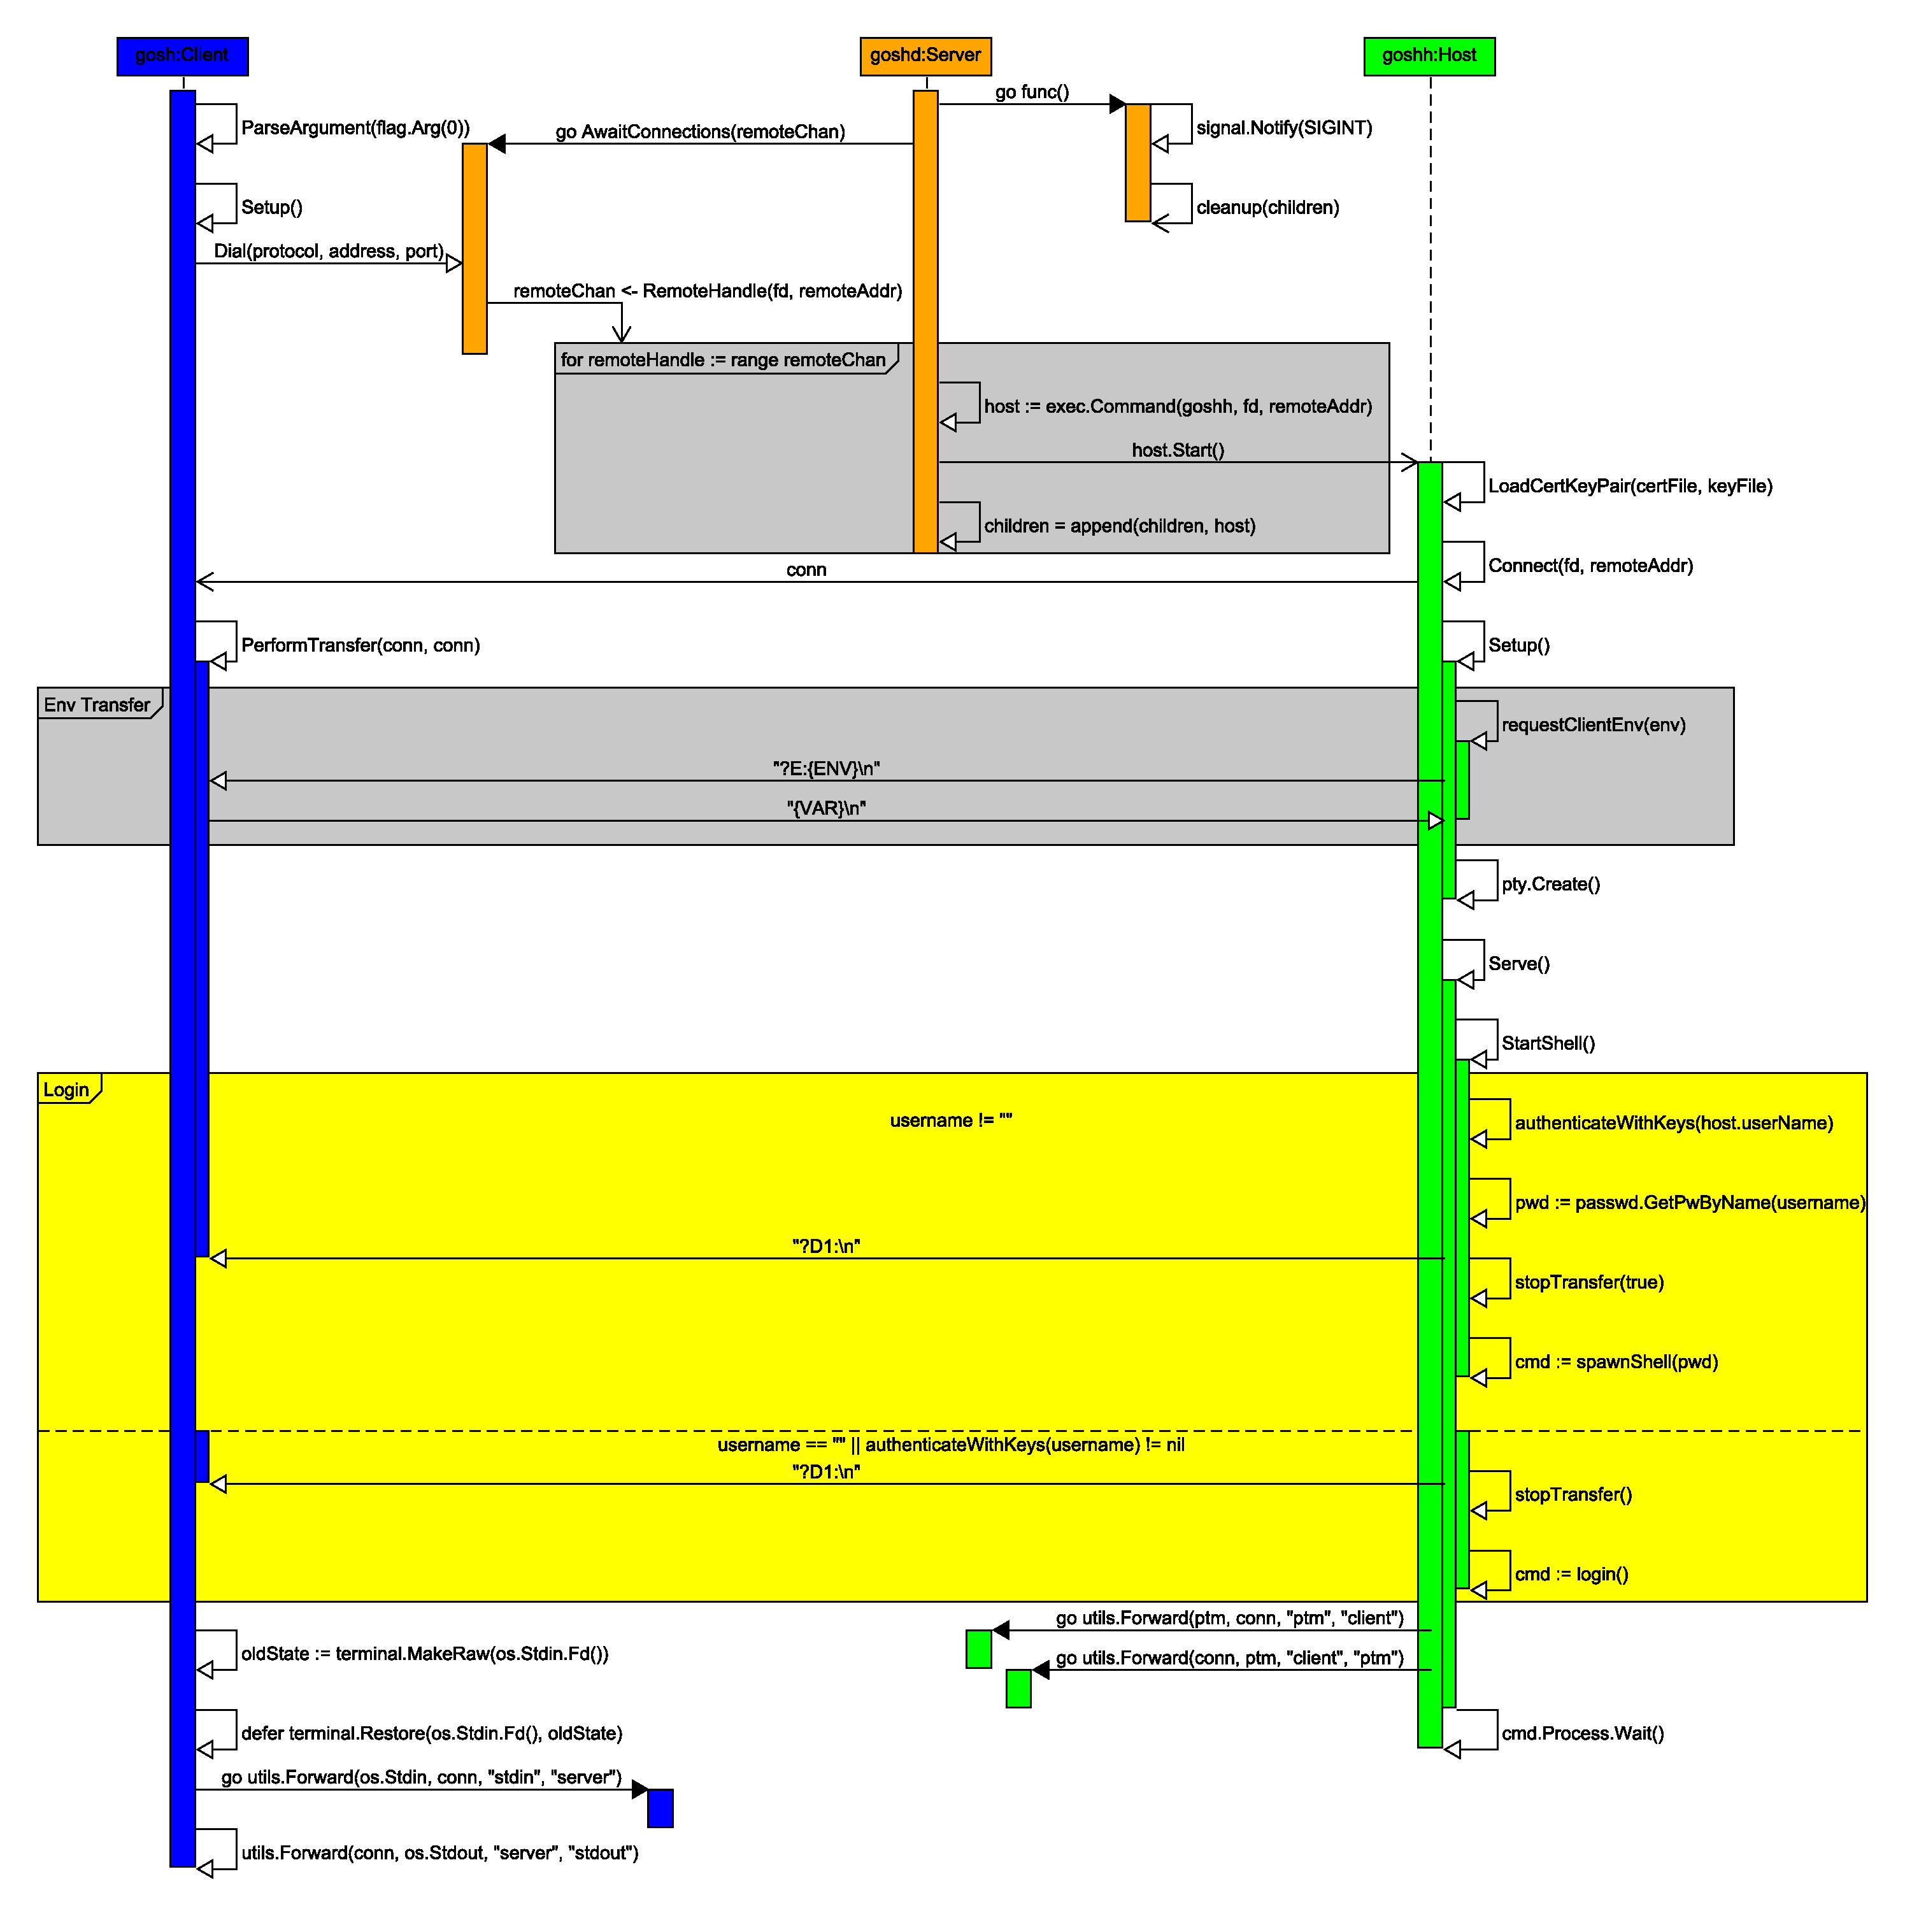
\includegraphics[width=\textwidth]{SequenceDiagramNew}
\caption{Sequence diagram of current implementation.}
\label{fig:SeqDiaCurrent}
\end{figure}

This new design of the \texttt{goshd} server calls the external binary \texttt{goshh} from the server process and lets it handle the connection itself. The server then asks for some environment variables from the client. Then the server tries to figure out whether the client can authenticate himself via keys. If authentication with keys is a viable option, it performs the key authentication according to \ref{sec:AuthViaKeys}. If it succeeds, it notifies the client of the authentication result. The host then spawns the user's \gls{shell} and forwards the traffic between the two.\\
If key authentication does not succeed, the host performs the classical authentication with user-password-credentials which also ends in spawning a user \gls{shell} if successful.\\
If the \gls{shell} exits or the host process receives an \gls{SIGINT}, it cleans up behind the exited \gls{shell} and exits as well.\\
The client performs the transfer of the environment variables until it receives the termination packet. Upon arrival of said packet, it prepares for the forwarding of the traffic between the user and the server. It does so by setting the \gls{terminal} in raw-mode and waits until the connections dies(it receives \texttt{EOF}) and then restores the \gls{terminal} to the default cooked state.


\chapter{Implementation}\label{chp:Implementation}
\notes{
\item (Beschreibt die Grundüberlegungen der realisierten Lösung (Konstruktion/Entwurf) und die Realisierung als Simulation, als Prototyp oder als Software-Komponente)
\item (Definiert Messgrössen, beschreibt Mess- oder Versuchsaufbau, beschreibt und dokumentiert Durchführung der Messungen/Versuche)
\item (Experimente)
\item (Lösungsweg)
\item (Modell)
\item (Tests und Validierung)
\item (Theoretische Herleitung der Lösung)
}
\section{Problems}\label{sec:Problems}
\subsection{Forking}\label{ssec:Forking}
To handle new established connections, it was deemed important to \texttt{fork} the process, as this duplicated the current process' memory and returns the \gls{PID}: 0 for the child process and a number greater than 0 for the parent to have the \gls{PID} of the child.\\
In theory, this should have enabled the program to use \gls{Go}s standard library capabilities to handle connections. However, there were several problems with this approach:

\subsubsection{Forking not supported}\label{sssec:ForkingNotSupported}
The \gls{Go} standard library does not support the classical \gls{C}-like forking. It only has a \texttt{syscall.ForkExec} method, which is documented as:
\begin{quote}
Combination of fork and exec, careful to be thread safe.
\end{quote}
But since it uses \texttt{exec} as well, it is the same as calling arbitrary binaries/scripts with the \texttt{exec.Cmd} function.\\
However: \gls{Go} has a feature called \gls{CGo}, which allows programs to call and interact with native \gls{C}-routines. This opens up the possibility of using \texttt{fork(2)}.

\subsubsection{Forking breaks Go objects}\label{sssec:ForkingBreaksGoObjects}
Forking with the functionality of \gls{CGo} does not solve the problem either. The reason is that after forking there are two programs with a \texttt{net.Conn} object. This lead to both connection objects being corrupted and turning unusable. Therefore, it was necessary to abandon the clean solution of forking and instead creating a new executable that can handle new connections by its own.

\subsubsection{Sharing Data with Child}\label{sssec:SharingDataWithChild}
The question then was: How can a process instantiate a child process and hand over all resources to it necessary for handling the new connection?\\
Since they are 2 separate processes now, they don't share any memory anymore. Hence the parent has to give the child the information about the connection via arguments. The most direct way to deal with this is to use \glspl{fd}, which can be passed as integer arguments to the child.

\subsubsection{Go Connection Cannot Be Transferred}\label{sssec:GoConnectionCannotBeTransferred}
Getting a \texttt{net.Conn} interface from a \gls{fd} is supported in \gls{Go} via:
\setlistingGo
\begin{lstlisting}[caption={Getting a \texttt{net.Conn} interface from a \gls{fd}},label=lst:ConnFromFD]
fd := uintptr(0) // Dummy fd
conn, err := net.FileConn(os.NewFile(fd, "conn"))
if err != nil {
	panic(err.String())
}
\end{lstlisting}

Getting the \gls{fd} from a connection is also possible:
\setlistingGo
\begin{lstlisting}[caption={Getting the \gls{fd} from a \texttt{net.Conn} object},label=lst:FDFromConn]
file, err := conn.(*net.TCPConn).File()
if err != nil {
	panic(err.String())
}
fd := file.Fd()
\end{lstlisting}

However: Creating a connection with the high-level \gls{API} of \gls{Go} and handing over the \gls{fd} to the child to derive a \texttt{net.Conn} object from it fails.\\
This had some implications for the project: The listener on the server could not be created with the high-level like:
\setlistingGo
\begin{lstlisting}[caption={\gls{Go}s high level \gls{API} for listener},label=lst:ListenForConn]
ln, err := net.Listen("tcp", ":8080")
if err != nil {
	// handle error
}
for {
	conn, err := ln.Accept()
	if err != nil {
		// handle error
	}
	go handleConnection(conn)
}
\end{lstlisting}

Instead the project had to rely on the low-level \gls{socket}. The \gls{x-package} \texttt{Unix} provides the necessary wrapper functions, which can be used instead.\\
The obvious drawback: Having to rely on a \gls{x-package} which is subject to change and not being able to use the higher-level methods which \textbf{are} part of the standard library.



\chapter{Results}\label{chp:Results}
\notes{\item (Zusammenfassung der Resultate)}

\chapter{Discussion And Prospects}\label{chp:DiscussionAndProspects}
\notes{
\item Bespricht die erzielten Ergebnisse bezüglich ihrer Erwartbarkeit, Aussagekraft und Relevanz
\item Interpretation und Validierung der Resultate
\item Rückblick auf Aufgabenstellung, erreicht bzw. nicht erreicht
\item Legt dar, wie an die Resultate (konkret vom Industriepartner oder weiteren Forschungsarbeiten; allgemein) angeschlossen werden kann; legt dar, welche Chancen die Resultate bieten
}

\chapter{Index}\label{chp:Index}
\bibliography{reference}\label{sec:Bibliography}
\newpage
\printglossary\label{sec:Glossary}
\newpage
\listoffigures\label{sec:ListOfFigures}
\newpage
\listoftables\label{sec:ListOfTables}
\newpage
\lstlistoflistings\label{sec:ListOfListings}
\newpage
\printglossary[title=SymbolGlossary,type=symbols]\label{sec:SymbolGlossary}
\newpage
\printglossary[title=Acronym Glossary,type=\acronymtype]\label{sec:AcronymGlossary}
\newpage
\printindex\label{sec:Index}

\appendix
\chapter{Appendix}\label{chp:Appendix}
\section{Project Management}\label{sec:ProjectManagement}
\notes{
\item Offizielle Aufgabenstellung, Projektauftrag
\item (Zeitplan) 
\item (Besprechungsprotokolle oder Journals)
}
\subsection{Official Statement of Tasks}\label{ssec:OfficialStatementOfTasks}
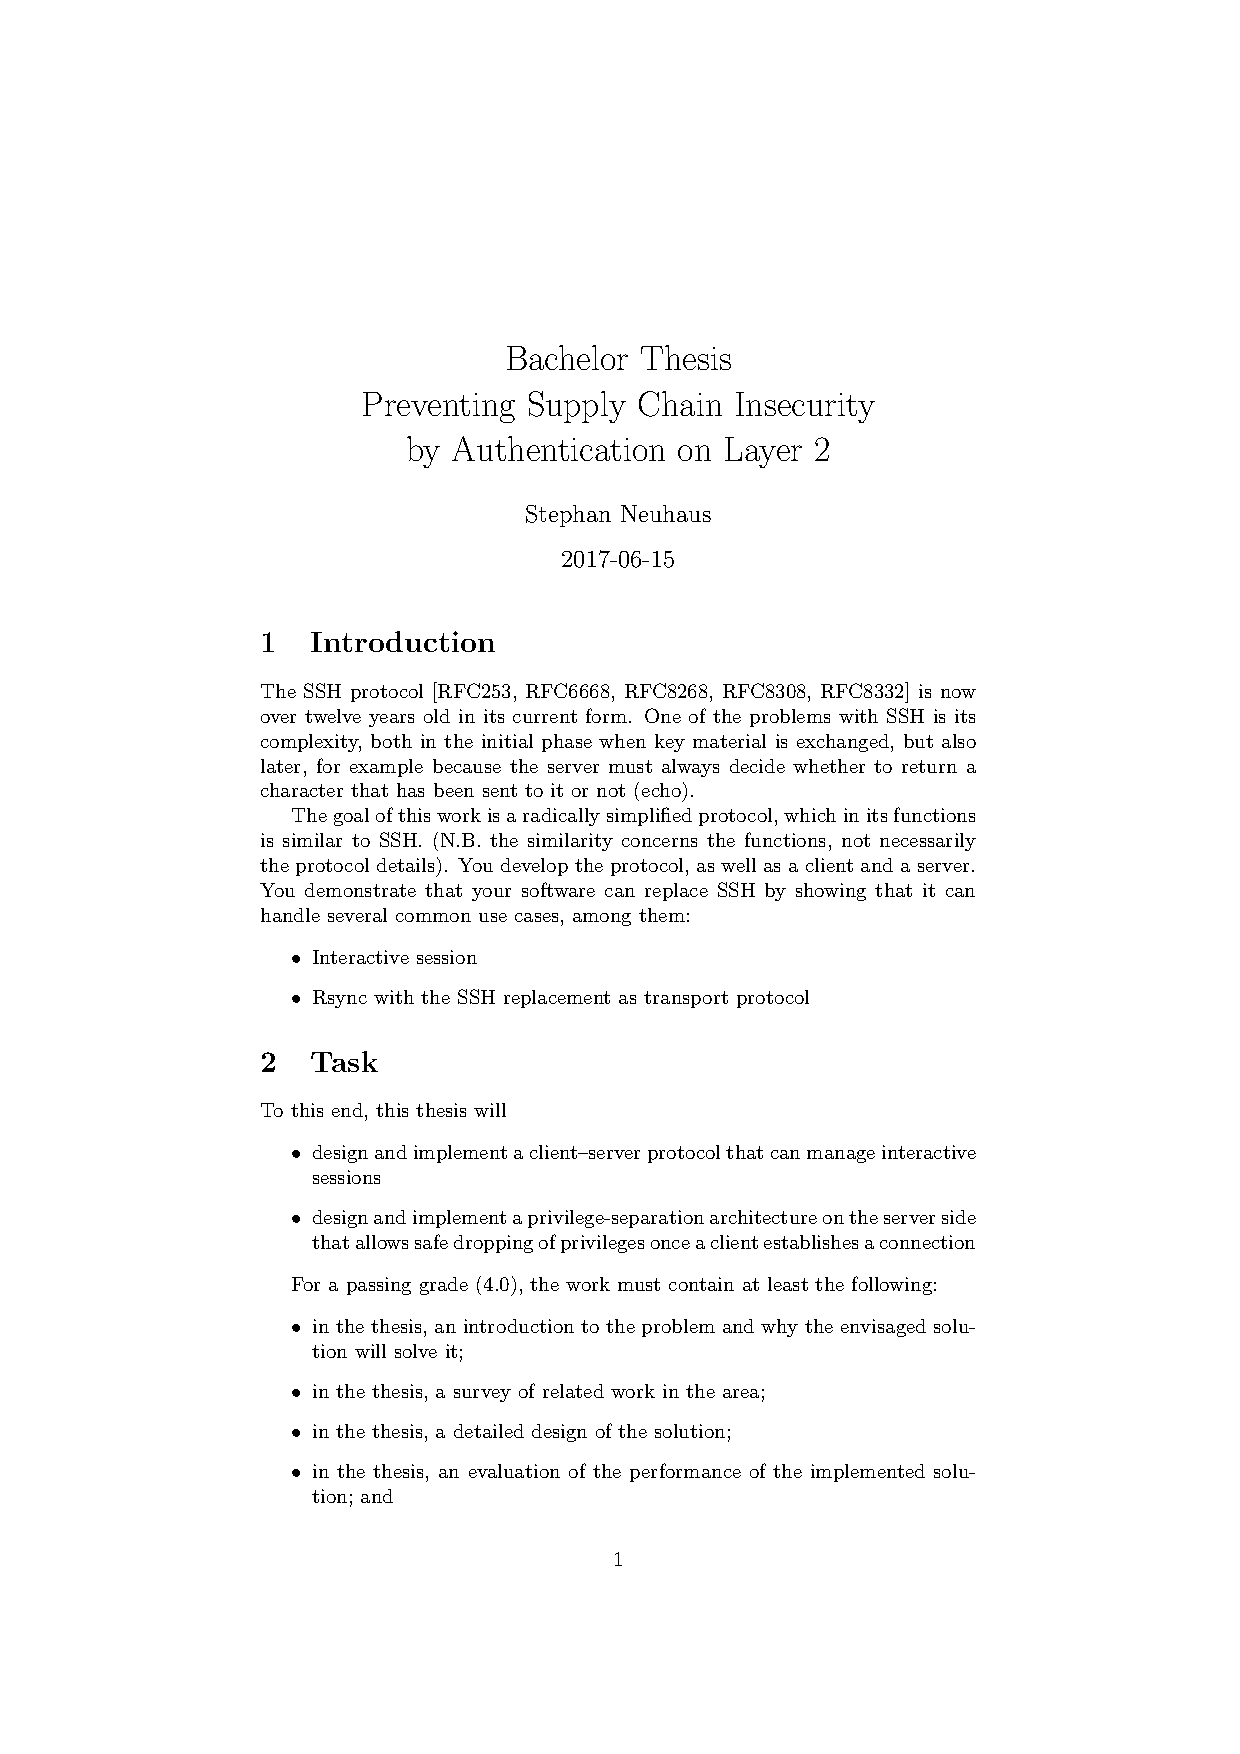
\includepdf[pages=-]{tasks.pdf}
\subsection{Project Plan}\label{ssec:ProjectPlan}
\includepdf[pages=-]{projectplan/Revised_project_plan.pdf}
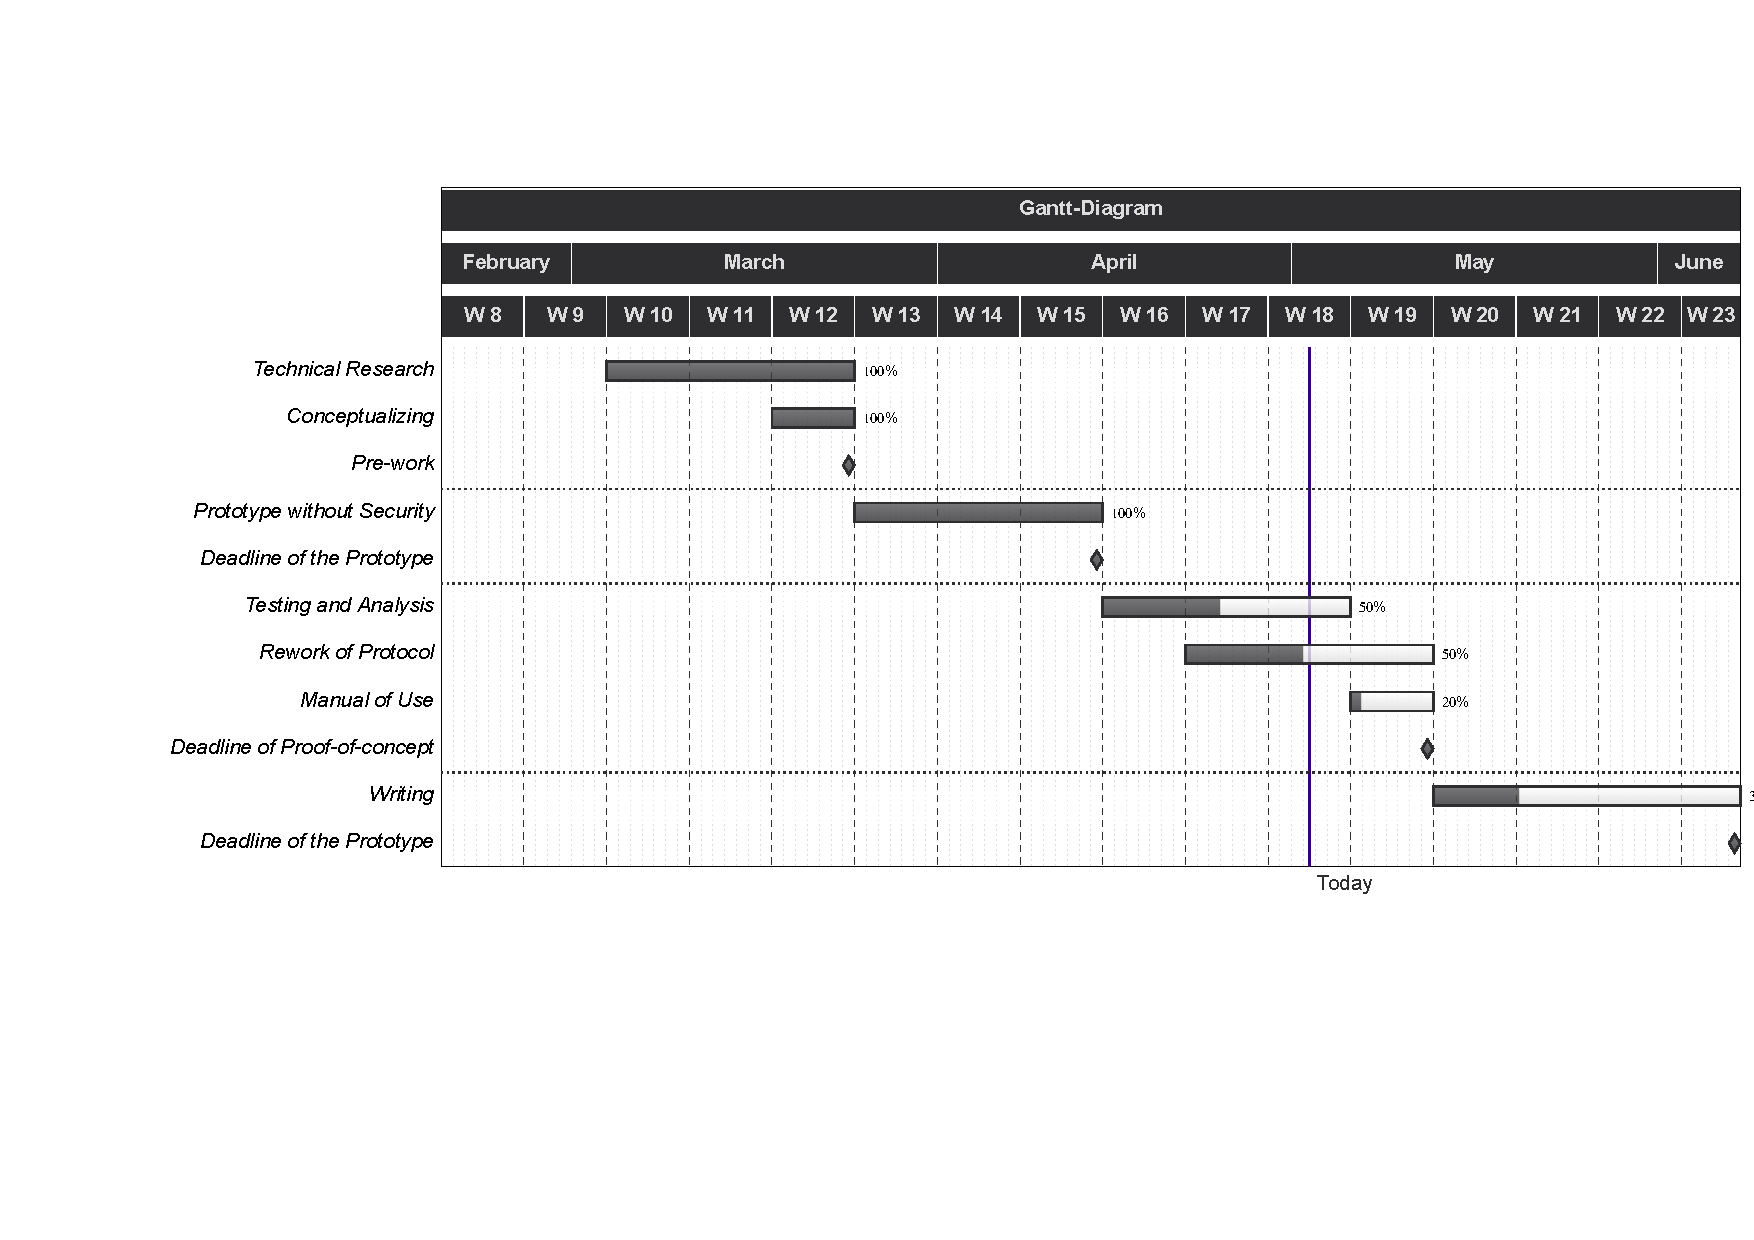
\includepdf[pages=-,landscape=true]{zhawGanttDiagram.pdf}
\subsection{Meeting Minutes}\label{ssec:MeetingMinutes}
The meeting minutes have a disruption in style and execution beginning from the 6th meeting. Reason for this is because in the beginning of the project, Mr Schwarz was responsible for keeping the minutes, but he opted out of the project.
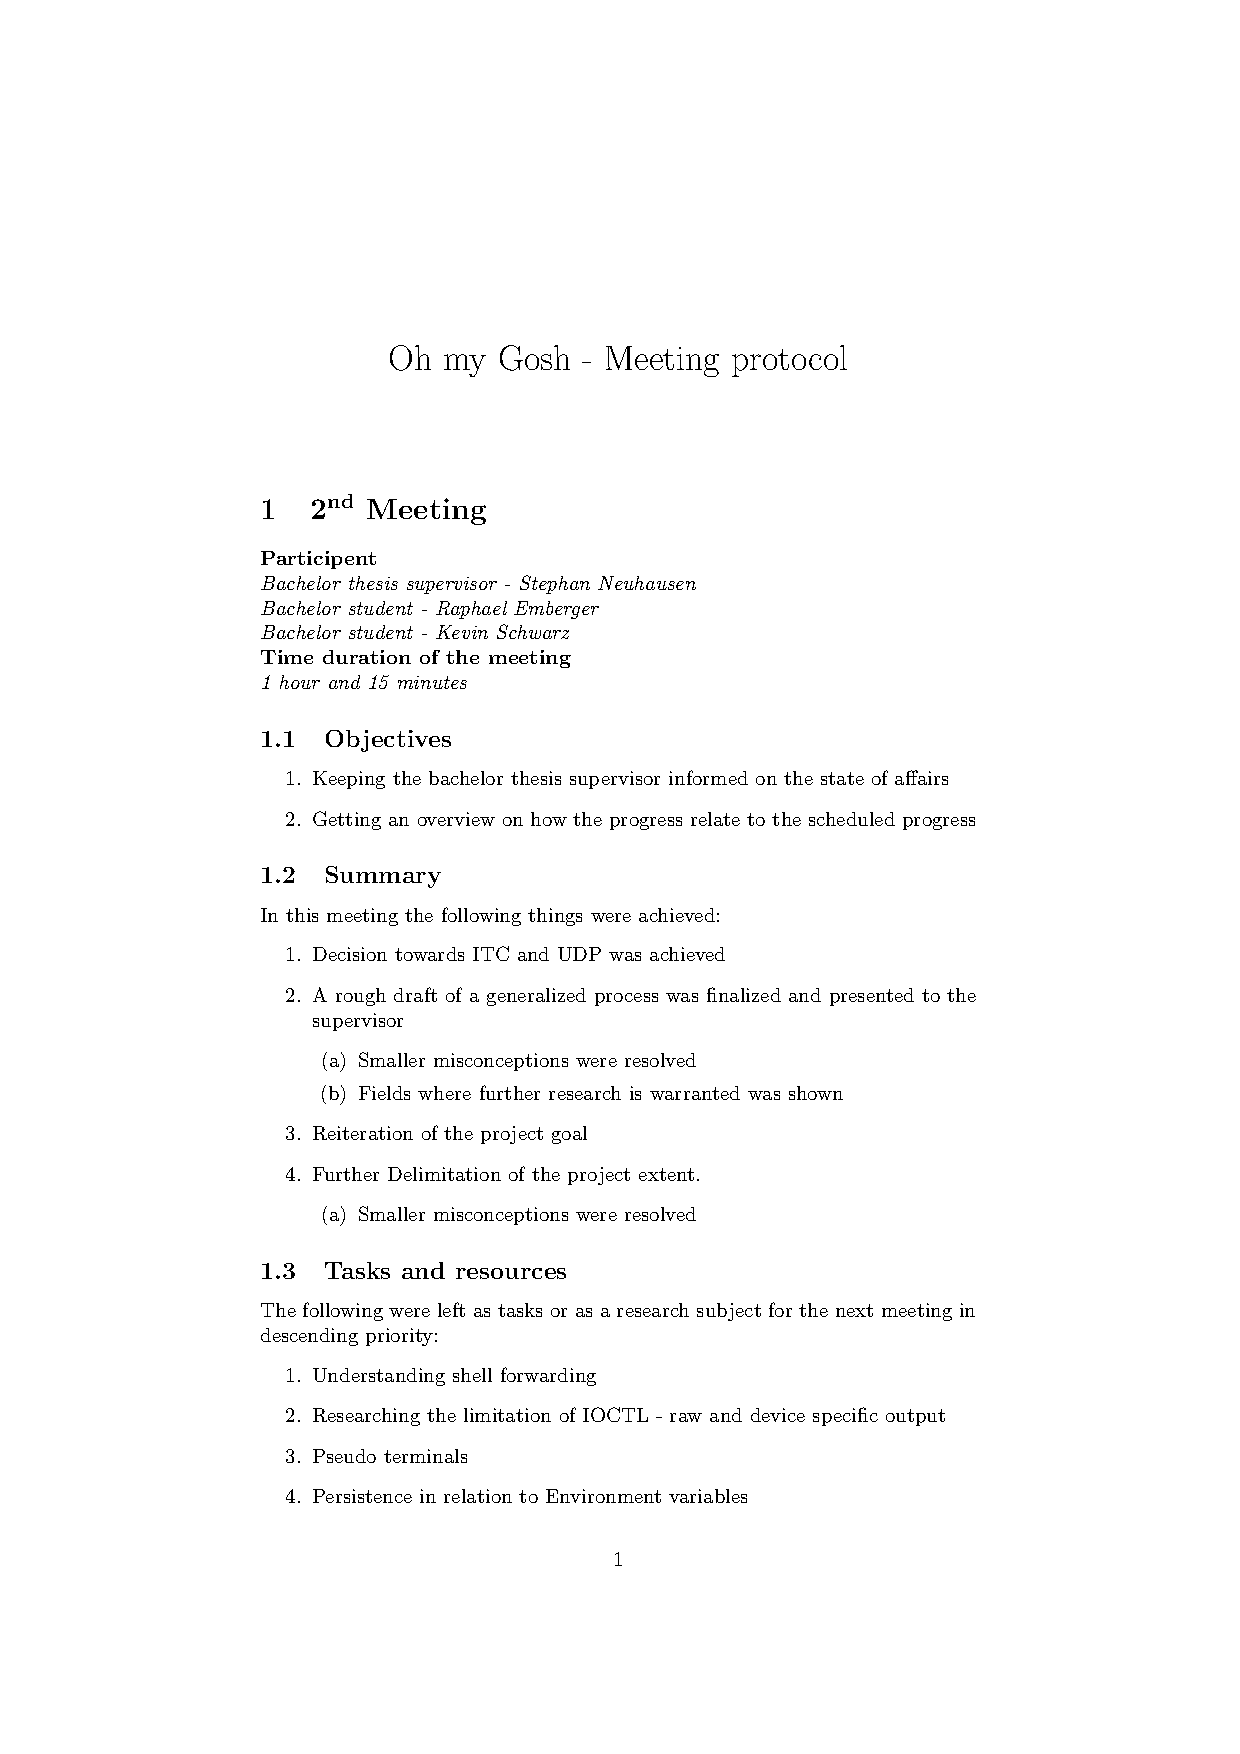
\includepdf[pages=-]{minutes/2nd_Meeting.pdf}
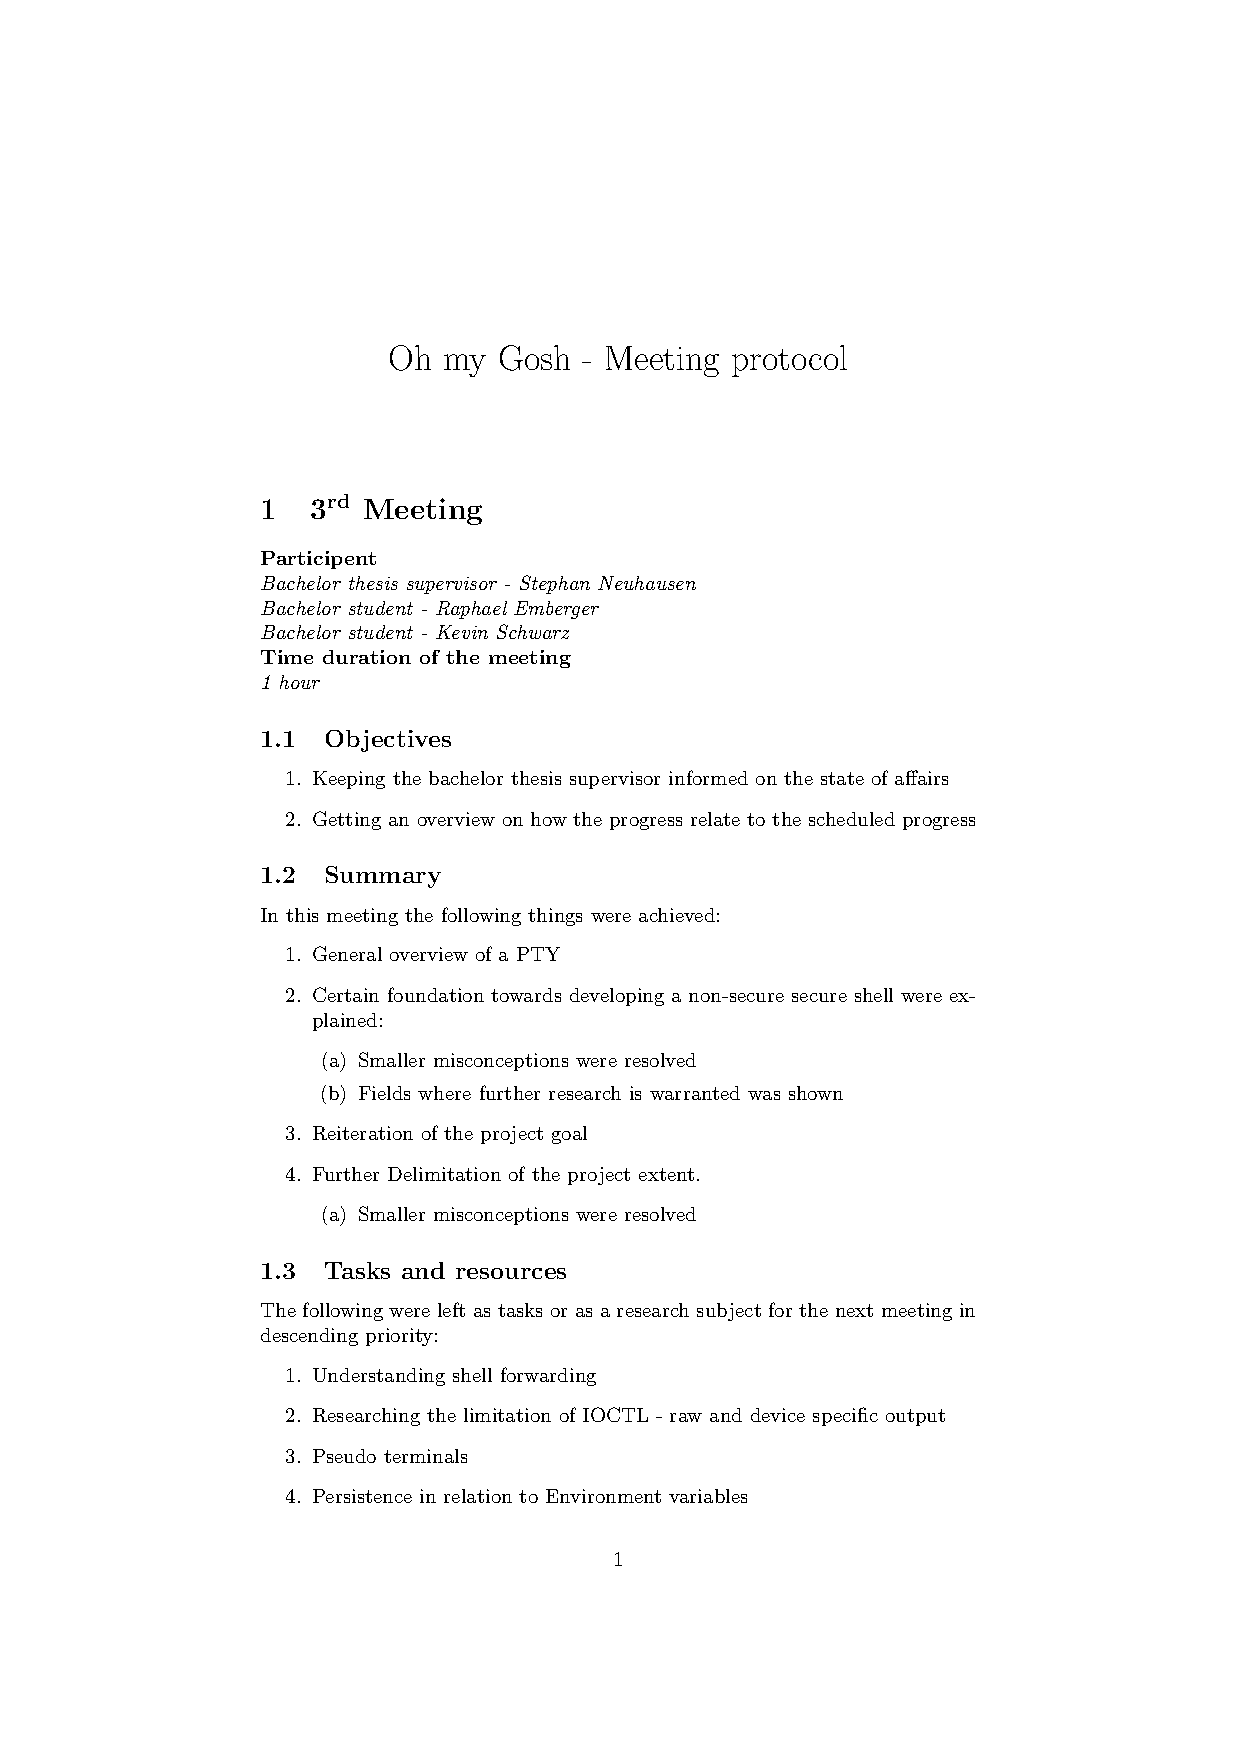
\includepdf[pages=-]{minutes/3rd_Meeting.pdf}
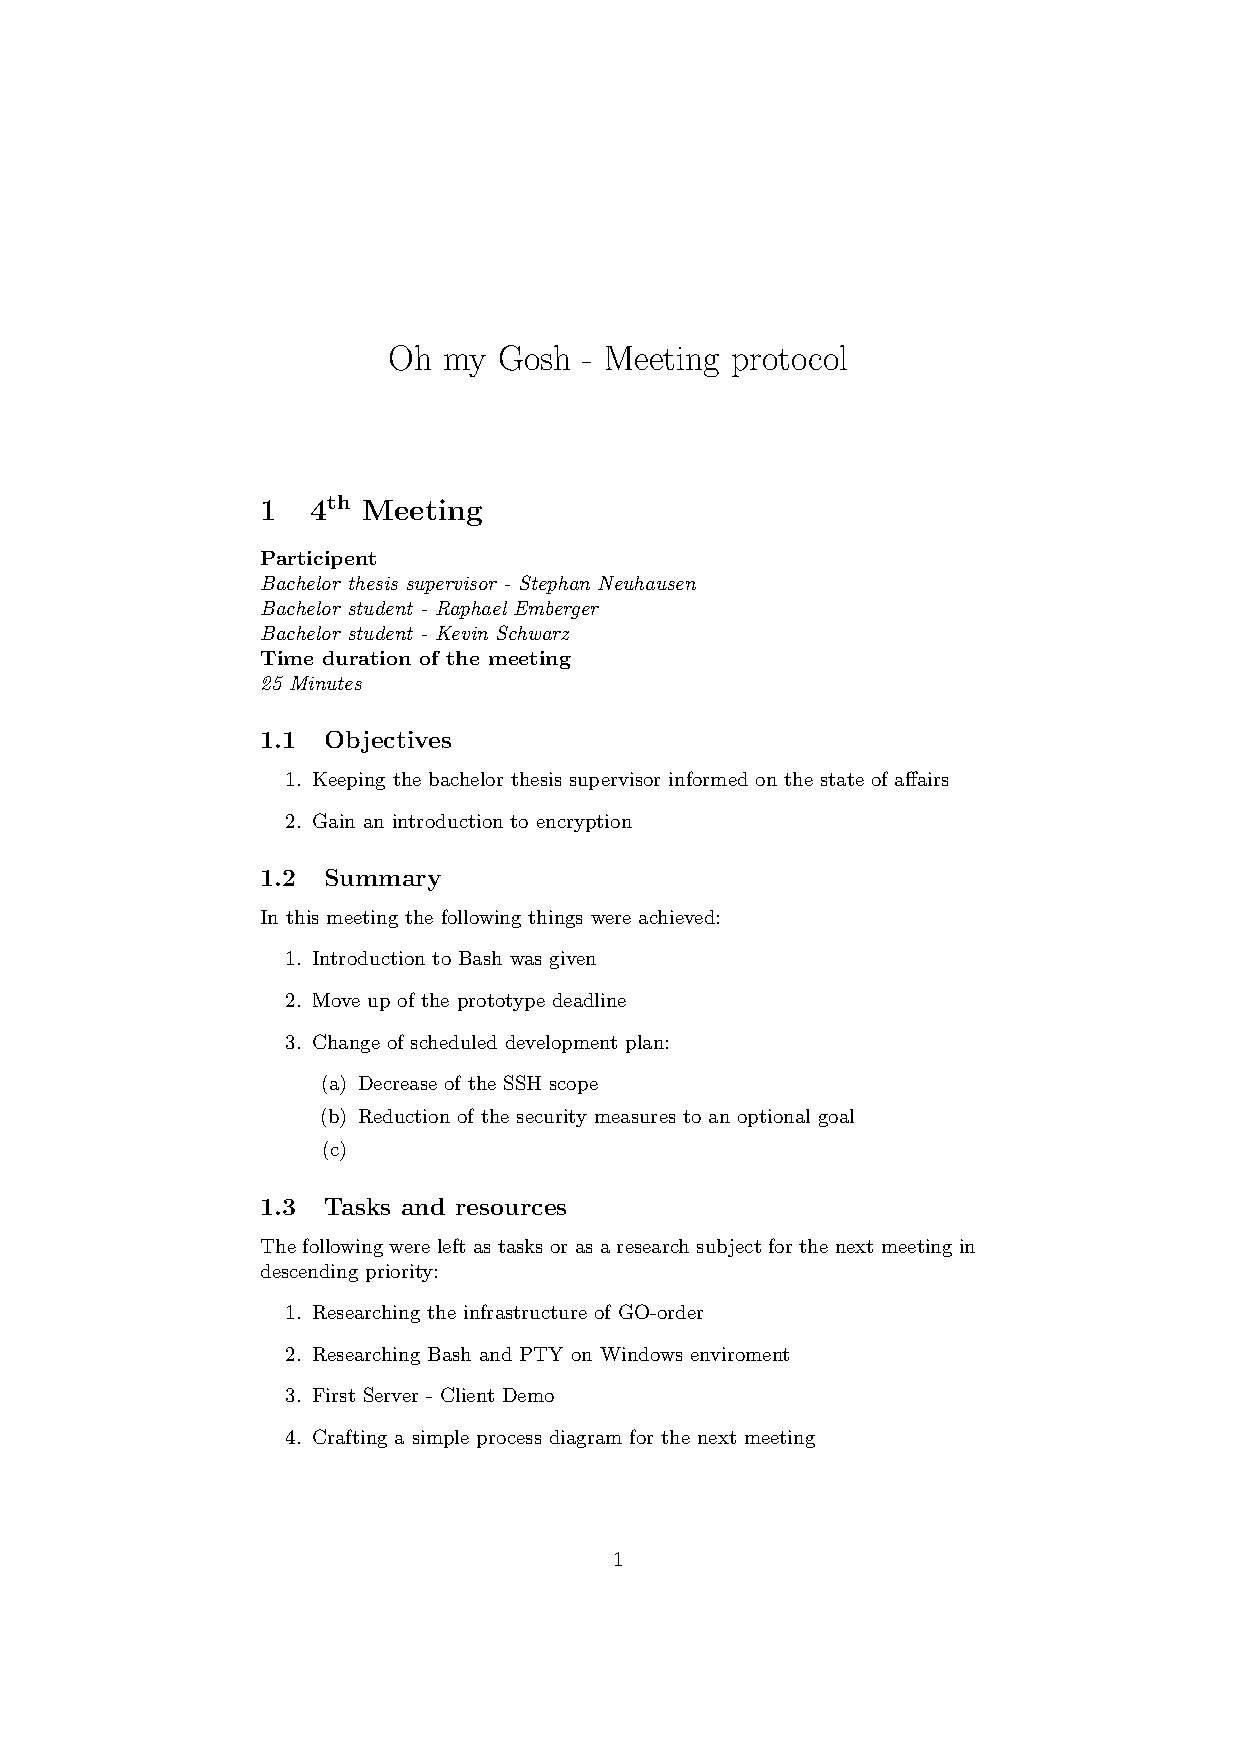
\includepdf[pages=-]{minutes/4th_Meeting.pdf}
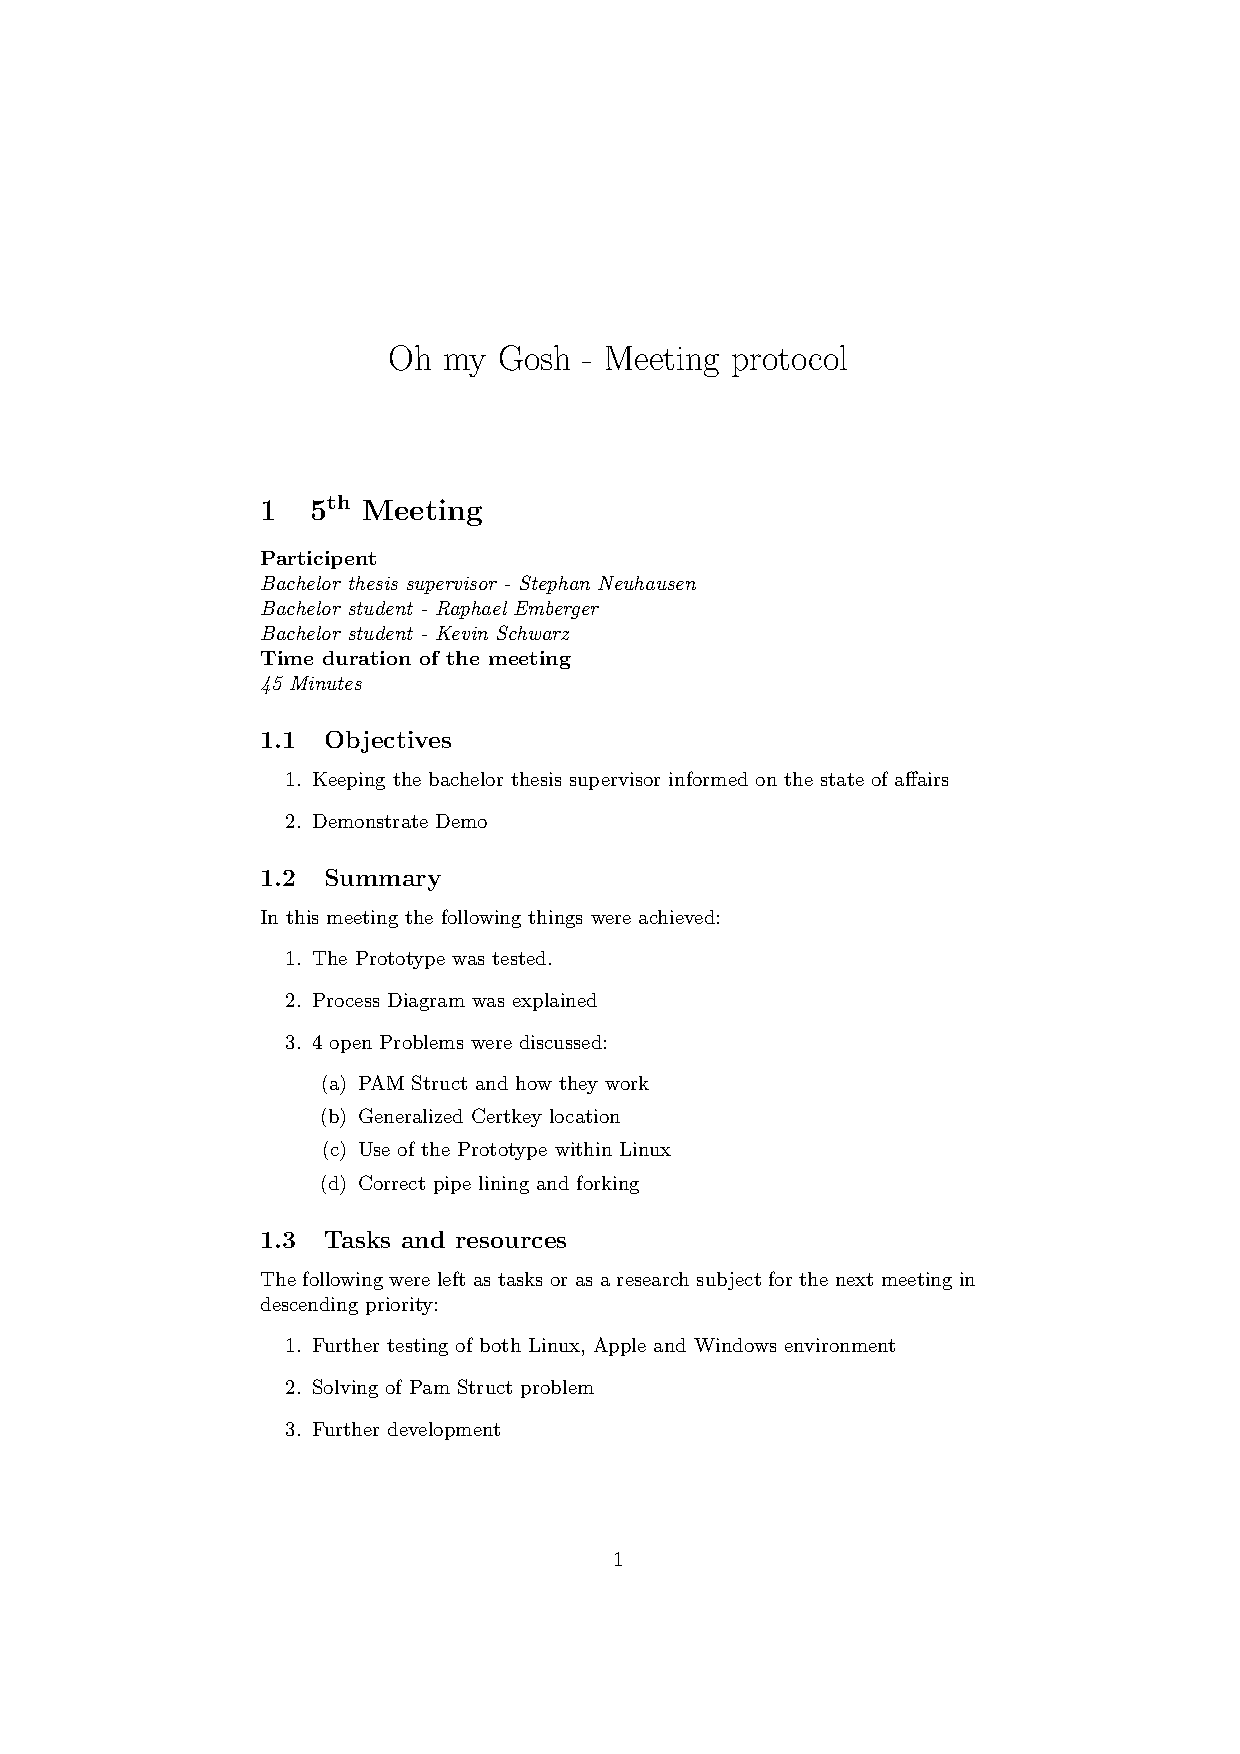
\includepdf[pages=-]{minutes/5th_Meeting.pdf}
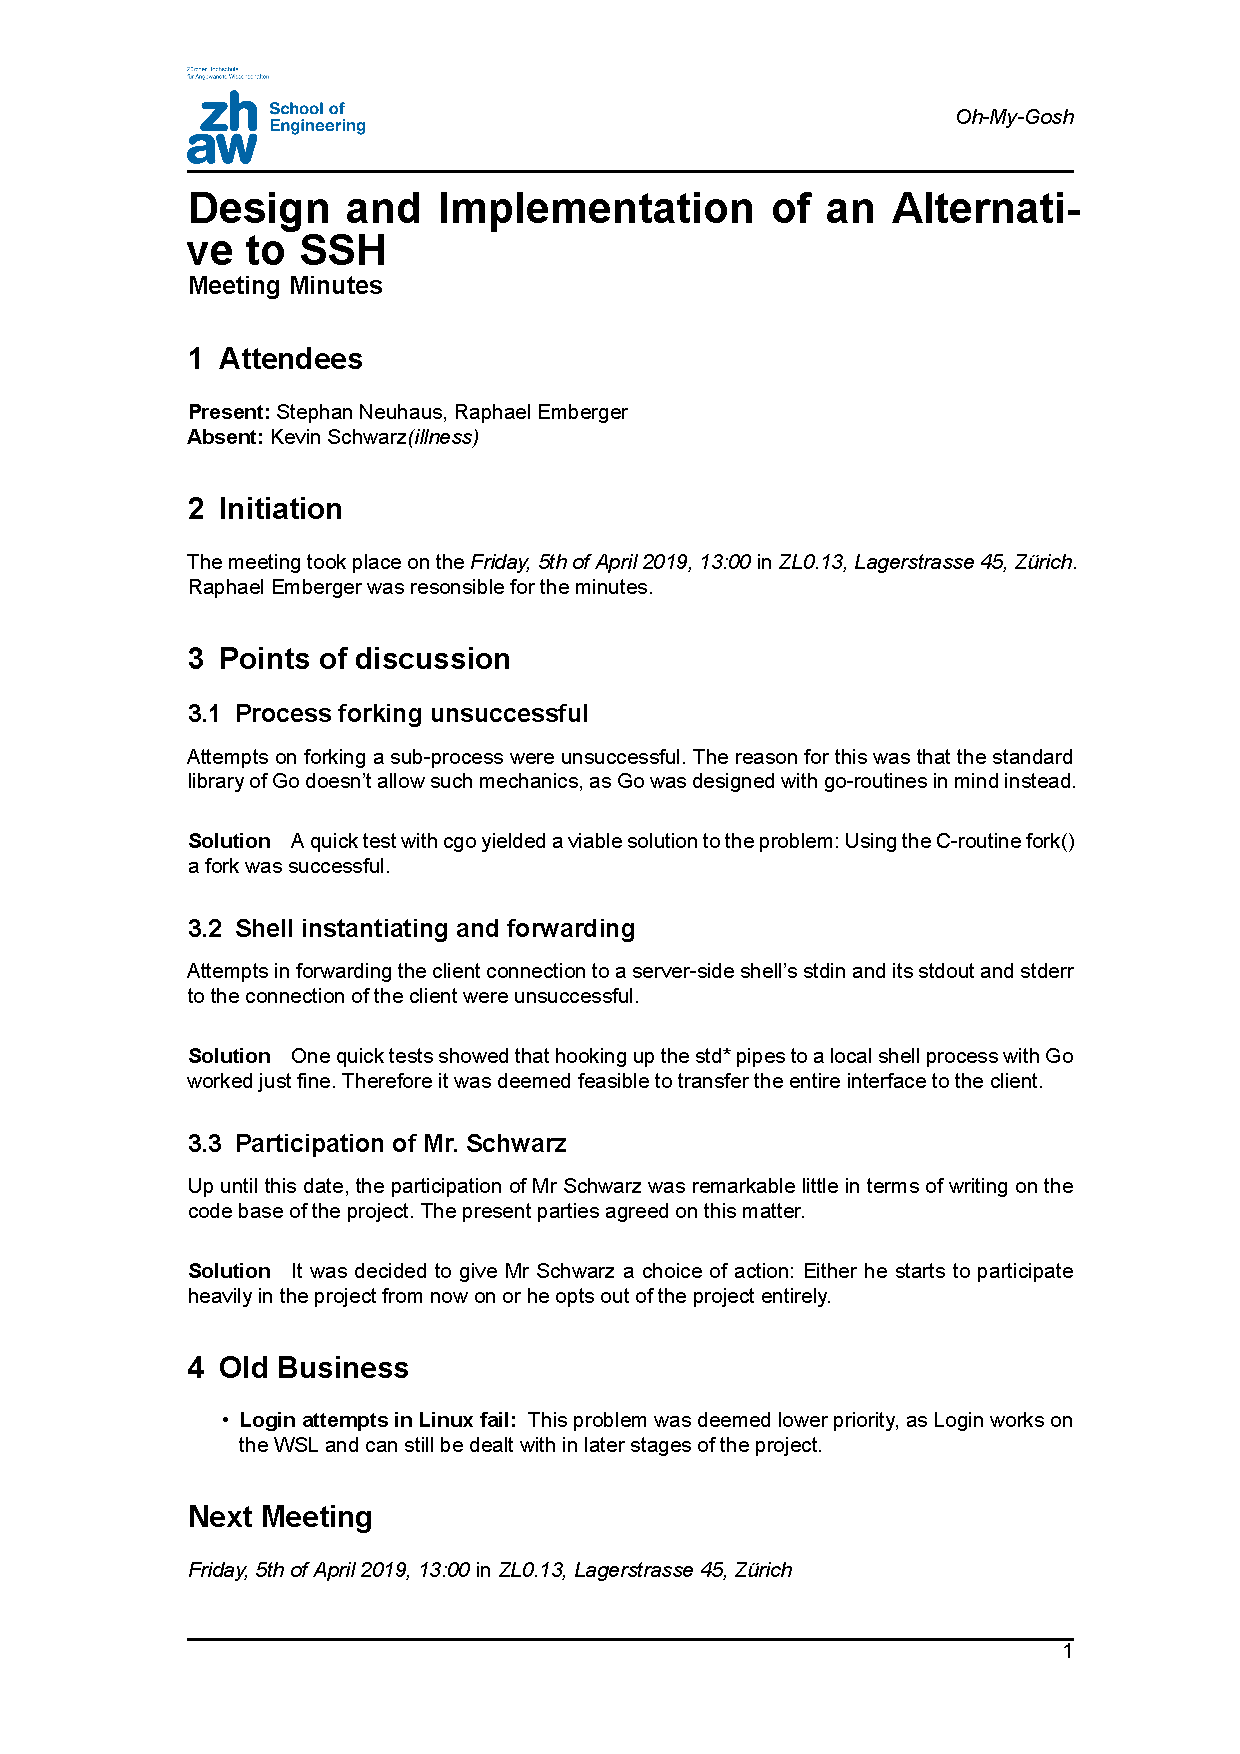
\includepdf[pages=-]{minutes/6th_Meeting.pdf}

\includepdf[pages=-]{minutes/7th_Meeting.pdf}

\includepdf[pages=-]{minutes/8th_Meeting.pdf}

\includepdf[pages=-]{minutes/9th_Meeting.pdf}

\includepdf[pages=-]{minutes/10th_Meeting.pdf}
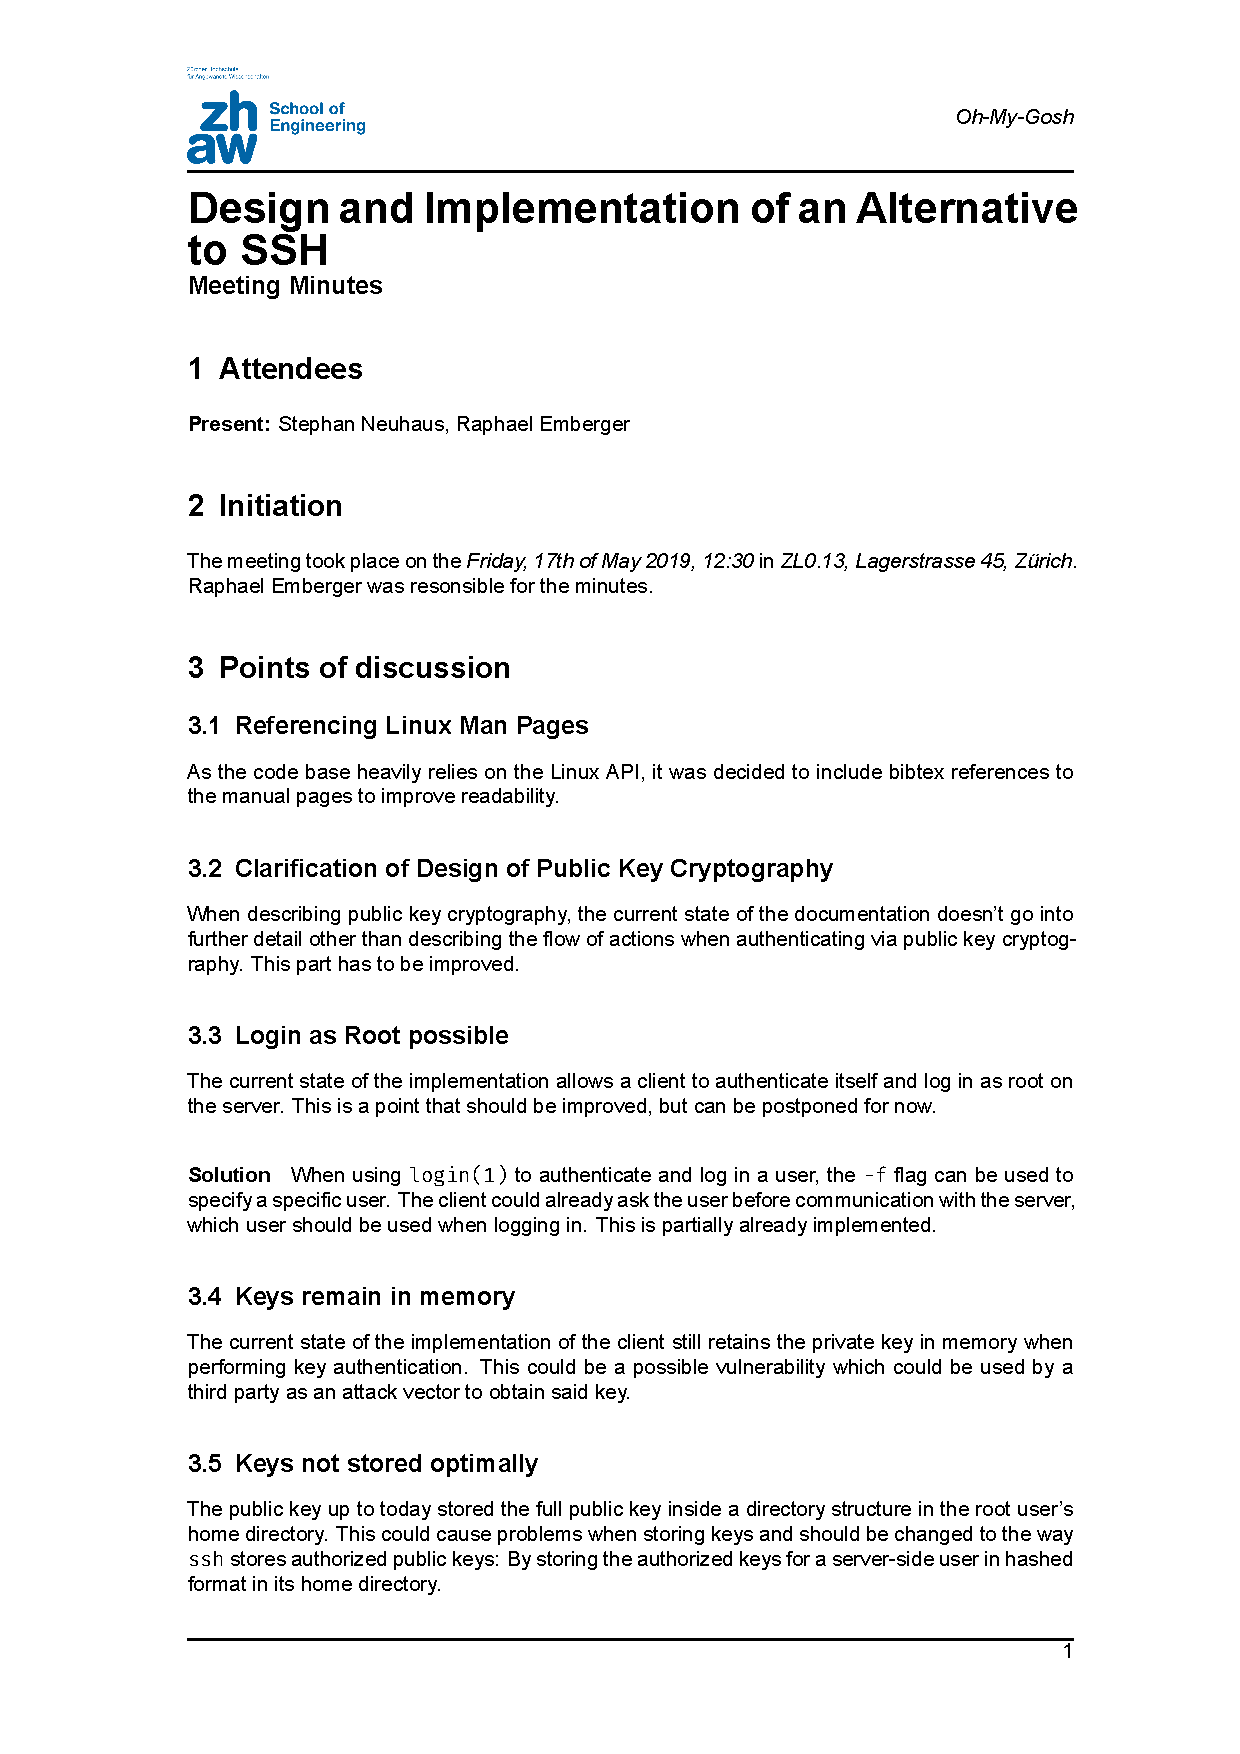
\includepdf[pages=-]{minutes/11th_Meeting.pdf}

\section{Others}\label{sec:Others}
\notes{
\item CD mit dem vollständigen Bericht als pdf-File inklusive Film- und Fotomaterial
\item (Schaltpläne und Ablaufschemata)
\item (Spezifikationen u. Datenblätter der verwendeten Messgeräte und/oder Komponenten)
\item (Berechnungen, Messwerte, Simulationsresultate)
\item (Stoffdaten)
\item (Fehlerrechnungen mit Messunsicherheiten)
\item (Grafische Darstellungen, Fotos)
\item (Datenträger mit weiteren Daten(z. B. Software-Komponenten) inkl. Verzeichnis der auf diesem Datenträger abgelegten Dateien)
\item (Softwarecode)
}
\end{document}
